\chapter{Robust motion planning with accuracy optimization via learned sensitivity metrics}\label{chap:sampNN}
\markboth{Robust MP with accuracy optimization via learned sensitivity metrics}{}% To set left/right header
\localtableofcontents \newpage

This last contribution introduces an enhanced version of the sensitivity-aware variants from Chapter~\ref{chap:samp}, incorporating the GRU-based architecture from Chapter~\ref{chap:NN} to mitigate the computational cost of solving thousands of \myglsentry{odes} in sampling-based contexts. 
Moreover, methods from Chapter~\ref{chap:samp} and the ones in the literature focus on computing robust trajectories but do not consider the problem of \emph{also} minimizing uncertainty tubes at a desired location for increasing the accuracy of specific tasks (e.g., insertion, grasping).
Therefore, in this chapter, a novel sensitivity-based cost function is introduced, differing from the one in Chapter~\ref{chap:samp}. 
Instead of minimizing sensitivity along the entire trajectory, it focuses on minimizing the radius of uncertainty tubes in relevant directions at desired states for the task at hand. 
Additionally, unlike Chapter~\ref{chap:samp}, where trajectory states were the sole optimization variables, this chapter also considers controller gains as optimization variables during the planning process.

With respect to these considerations, the contribution of this chapter is twofold:
\begin{enumerate}
    \item A computationally efficient version of the \myglsentry{samp} variants (see Chapter~\ref{chap:samp}) is proposed, relying on a Gated Recurrent Unit neural network (GRU)\cite{cGRU} (see Chapter~\ref{chap:NN}), which quickly and accurately estimates time-varying uncertainty tubes and control input profiles along trajectories.
    A general method for incorporating this network into a sampling-based tree planners is presented to predict uncertainty tubes and control inputs along trajectories.
    \item Based on this new planner variants, a comprehensive framework is proposed that plans robust trajectories and locally optimizes them, along with the controller gains, to maximize accuracy at desired states of the planned trajectory for any system/controller.
\end{enumerate}

This chapter is structured as follows: Section~\ref{sec:RASAMP} introduces the integration of the GRU-based architecture within sampling-based planners and details the process of accuracy optimization.
Then, Section~\ref{sec:SimuResults} demonstrates the approach efficiency through simulation results.
Finally, these contributions are experimentally validated in Section~\ref{sec:Experimental} through two challenging scenarios illustrated in Figure~\ref{fig: Missed and succes}, which demonstrate the application to a quadrotor model in experimental settings involving uncertain parameters. 
The scenarios include: (i) robust navigation through a narrow window, and (ii) an in-flight ring-catching task. 
These experiments highlight the robustness and accuracy of the proposed framework under parameter uncertainties in the robot model.

This chapter is associated to the following publication in RA-L 2024~\cite{cRAL}: Wasiela, S., Cognetti, M., Giordano, P. R., Cortés, J., and Simeon, T. (2024). "Robust Motion Planning with Accuracy Optimization based on Learned Sensitivity Metrics." In IEEE Robotics and Automation Letters (RA-L).

\section{Robust and accurate planning framework}\label{sec:RASAMP}

This section presents the workflow of the meta-algorithm used to plan robust trajectories, which are then locally optimized for accuracy at specified desired states. 
The method consists of two stages: 
\begin{enumerate}
    \item First, it generates a robust trajectory based on a Deep learning-based Sensitivity-Aware Motion Planner (DeepSAMP) -- explained in Sect.~\ref{sec:RSAMP} -- that utilizes the GRU-based computation of the uncertainty tubes.
    \item Second, it optimizes the accuracy at some given states along this trajectory by minimizing the size of the uncertainty tubes at these locations.
\end{enumerate}

The motivation behind the second stage is to improve the accuracy of the planned robust trajectory for tasks -- e.g., pick-and-place or insertion tasks -- where minimizing the deviation from the nominal trajectory is important only at specific designed locations, as for picking the ring in Figure~\ref{fig: Missed and succes}.

The workflow of the method is presented in Algorithm~\ref{alg:RA-SAMP}. 
It takes as input (line 1) a list of desired states $list_{d} = (q_{d}^0, \dots, q_{d}^n)$ for which the accuracy should be optimized, and the initial controller gains vector $k_{c}^{init}$ considered constant all along the trajectory.
The role of the controller gains are further discussed in Section~\ref{sec:AccOptSimu}.

\begin{algorithm}[htp]
\caption{Robust and Accuracy Optimization [$list_{d}, k_{c}^{init}$]}\label{alg:RA-SAMP}
\begin{algorithmic}[1]
\State $\q_d^{tot} \gets \emptyset;$
\For {($i=1;\ i< len(list_{d});\ i=i+1$)}
    \State $\q_d^{tot} \gets \q_d^{tot} + $DeepSAMP$(list_{d}(i-1),list_{d}(i));$
\EndFor
\State $\left \{ \q_d^{tot}, k_{c}^{opt} \right \} \gets $A-Optim$(list_{d},\q_d^{tot}, k_{c}^{init});$
\State \textbf{return} $\left \{ \q_d^{tot}, k_{c}^{opt}  \right \}$;
\end{algorithmic}
\end{algorithm}

The first step of the algorithm consists of generating robust trajectories between successive desired states in the list (line 3 of Algorithm~\ref{alg:RA-SAMP}) by means of a deep learning-based sensitivity-aware motion planner variant called DeepSAMP (explained in Section~\ref{sec:RSAMP}) that uses the learning approach presented in Chapter~\ref{chap:NN}.
These trajectories are concatenated into a global one $\q_d^{tot}$, connecting all the desired states of $list_{d}$ (lines 2-5 in Algorithm~\ref{alg:RA-SAMP}). 

The trajectory from DeepSAMP is locally modified by A-Optim (line 6 in Algorithm~\ref{alg:RA-SAMP}), aiming at optimizing the accuracy at specific desired states along the trajectory. 
This algorithm iteratively samples both the trajectory from DeepSAMP and the controller gains, adjusting the former to minimize uncertainty at these states. 
Indeed, as demonstrated in~\cite{AliIROS}, optimizing both factors concurrently results in minimizing the uncertainty.
The algorithm produces two offline outputs: $(i)$ a robust desired trajectory $\q_d^{tot}$ optimized for accuracy at the desired states, and $(ii)$ the optimized controller gains vector $k_{c}^{opt}$, considered constant throughout the trajectory.

\subsection{Deep Sensitivity-Aware Motion Planner (DeepSAMP)}\label{sec:RSAMP}

For clarity in the pseudo-code, the temporal notation is omitted in this section. 
Thus, bold symbols refer to time-dependent vectors (e.g., $\q_d$ represents a desired trajectory, $\Rq$ stands for the uncertainty tube radii along a trajectory, etc.), while non-bold symbols represent instantaneous vectors (e.g., $q^{rand}$ denotes a random state, and $h_0$ represents the initial hidden state of the GRU at a given state vector, etc.).

\subsubsection{General method}

This section explains how the deep learning method presented in Chapter~\ref{chap:NN} can be incorporated into any sampling-based tree planner in order to create \gls{deepsamp} variants, which use the learned model to predict uncertainty tubes.
As highlighted before, a key challenge in computing such tubes for a given trajectory lies in the high computational cost of numerically integrating the dynamics of $\bPi(t)$ and $\bTheta(t)$.
Additionally, when extending the tree and computing these sensitivity matrices, various initial conditions (such as the initial control input, $\bPi_0$, etc.) need to be incorporated into the tree nodes (as outlined in Chapter~\ref{chap:samp}).

This problem is addressed thanks to the GRU network, which naturally encodes this information in its ``memory'' terms, i.e., the so-called hidden state (see~\cite{cGRU}).
An interesting feature of the \myglsentry{deepsamp} variants is to leverage this latent state to embed the initial conditions into each node analogous to the \myglsentry{odes} initial conditions mentioned in Chapter~\ref{chap:samp}. 
This enables the reuse of the updated initial conditions for predictions in future extensions.
Note that a hidden state $h$ is unique according to its parent as the \myglsentry{odes} initial conditions.
Therefore, its use is only applicable to tree-based planners, where each node has a single parent.

\subsubsection{Deep Sensitivity-Aware RRT (DeepSARRT)}

This section proposes a deep learning-based sensitivity-aware variant of the \myglsentry{rrt}~\cite{cRRT}, denoted \gls{deepsarrt} as a particular instance of \myglsentry{deepsamp}, and presented in Algorithm~\ref{alg:ExtensionExample}. 
It demonstrates how to integrate the GRU hidden state and tube predictions within a standard RRT planner~\cite{cRRT}.
It is important to note that this approach, using GRU hidden state and tube predictions, can be similarly applied to other tree-based planners. 
For instance, in the results presented in Section~\ref{sec:RobustPlanSimu}, a deep learning-based sensitivity-aware variant of the \myglsentry{rrtstar}~\cite{cRRTstar} implementation, denoted \myglsentry{deepsarrt*}, leverage the same principle presented here.

First, \myglsentry{deepsarrt} performs the standard RRT procedure (lines 1-5) that produces a local desired trajectory $\q_d$ between a sampled state (${q}^{rand}$) and its nearest state (${q}^{near}$) in the tree. 
Then, the starting hidden state (as for $h_{0}$ of the GRU) is recovered from the tree node (line 6).
Such initial condition is used together with the above-mentioned desired trajectory by the GRU that returns all the radii and the control inputs profiles ($\Rq,\Ru,\u$), together with the final hidden state $h_{F}$ to be reused as initial condition in subsequent iterations (line 7).
Next, an initial filter is applied using the predicted control inputs and uncertainty tubes, with a robust control input check for saturation (line 8).
The nominal trajectory is then computed (line 9). 
At this stage, the control inputs are recomputed in a closed-loop manner w.r.t. the desired trajectory $\q_d$, even though these control inputs were initially predicted by the GRU.
However, directly using the predicted control inputs in an open-loop manner could lead to unsuitable nominal trajectories due to the accumulation of prediction errors over time in the simulation process.
Then, for each state of the nominal trajectory $\q_{n}$, the function \emph{IsStateRobust} (line 10) performs a robust collision checking by using the uncertainty radii.
If the extension is valid, the final state of the desired trajectory is inserted in the tree as a new node, embedding at the same time the final hidden state $h_{F}$ to be reused as initial condition in next iterations (line 10-12).
Finally, the algorithm returns a global trajectory connecting ${q}^{init}$ and ${q}^{goal}$ if one exists in the tree (lines 15).

Note that, unlike the \myglsentry{samp} variants discussed in Chapter~\ref{chap:samp}, which perform the robust feasibility check in a single step, the operation is decoupled here. 
This approach first leverages the predicted control inputs and associated tubes to apply an initial filtering stage, as this step is less computationally expensive than the subsequent nominal trajectory simulation and robust collision checking.

\begin{algorithm}[htp]
\caption{\myglsentry{deepsarrt} [$q^{init}, q^{goal}$]}\label{alg:ExtensionExample}
\begin{algorithmic}[1]
\State $T \gets$ InitTree$({q^{init}, q^{goal}});$
\While{\textbf{not} StopCondition$(T, {q^{goal}})$}  
    \State ${q^{rand}} \gets $Sample()$;$
    \State ${q^{near}} \gets$ Nearest$(T,{q^{rand}});$
    \State $\q_d \gets$ Steer$({q^{near}},{q^{rand}});$
    \State $h_{0} \gets $GetNodeConditions$({q^{near}});$
    \State $\left \{\Rq,\Ru,\u, h_{F} \right \} \gets $GRU$(\q_d,h_{0});$
    \If {$IsControlRobust(\Ru,\u)$}
        \State $\q_{n} \gets $SimulateExecution$(\q_d);$
        \If {$IsStateRobust(\Rq,\q_{n})$}
                \State SetNodeConditions$({q^{rand}}, h_{F});$
                \State AddNewNode$(T, {q^{rand}});$
                \State AddNewEdge$(T, {q^{near}}, {q^{rand}});$
        \EndIf
    \EndIf
\EndWhile
\State \textbf{return} GetTrajectory$(T, q^{init}, q^{goal})$;
\end{algorithmic}
\end{algorithm}

\subsection{Robust local accuracy optimization \emph{(A-Optim)} }\label{sec:AOptim}

This section introduces robust local optimizer variants, highlighting their capability to address accuracy-related costs effectively.

\subsubsection{Cost function}\label{sec:AOptimCost}

The application of a local optimization method at this level is justified by the cost function considered in order to optimize the accuracy at desired states. 
Indeed, the cost of a desired trajectory $\q_d$ is defined as:
\begin{equation}\label{eq: cost}
    c(\q_d) = w_1\mathbb{E}[L] + w_2\mathbb{V}[L], \quad L = \left[\lambda_{0} ... \lambda_n \right]
\end{equation}
with $\mathbb{E}[L]$ and $\mathbb{V}[L]$ the mean and the variance of $L$, where $\lambda_k$ is the p-norm of the radii of interest in the $k$-th state in the $list_{d}$ of Section~\ref{sec:RASAMP}, and $w_1, w_2$ are user-defined weights.
The variance is considered in this cost function so that the minimization of a radius at a given point does not lead to the growth of another radius at another waypoint.
As the cost function of Chapter~\ref{chap:samp}, this function is neither additive (i.e., considering two trajectories ($\q_{d,1}(t), \q_{d,2}(t)$), the cost of their concatenation $c(\q_{d,1}(t)|\q_{d,2}(t)) \neq c(\q_{d,1}(t)) + c(\q_{d,2}(t))$), nor monotonic. 
Therefore, it is unsuitable for global optimization using sampling-based motion planners like~\cite{cRRT,cRRTstar}, since they require additive and monotonic objective functions.
Given that the analytical expression of the cost function derivatives is unavailable, the accuracy optimization in A-Optim must be conducted using a derivative-free method.
In the following section several robust variant derivative-free algorithms are proposed to maintain the robustness of the initial trajectory computed by the \myglsentry{deepsamp} variant.

\subsubsection{Algorithms}

This thesis considers four robust sensitivity-aware local variants for optimizing the aforementioned cost function, aiming to identify the most suitable approach for optimizing a punctual cost function while appropriately scaling its complexity to the robust feasibility check described in Chapter~\ref{chap:samp}. 
It is important to note that none of the proposed robust variants utilize the deep learning method introduced in Chapter~\ref{chap:NN}, as the trajectories encountered during this local optimization process differ significantly from those in the training set.
Also note that in this section, only the trajectory states are optimization variables. 
The addition of controller gains in the optimization variables, as mentioned in the general framework (see Section~\ref{sec:RASAMP}), is detailed in Section~\ref{sec:AccOptSimu}.

\paragraph{Shortcut}

The first variant is the robust sensitivity-aware variant of the shortcut algorithm~\cite{cShortcut} presented in Chapter~\ref{chap:samp}.
This variant offers the advantage of a straightforward implementation, as it simply samples two states from the current best trajectory, attempts a new connection between them, and conducts a single robust feasibility test per algorithm iteration.
While this algorithm is computationally efficient, it is constrained by sampling on the current trajectory, limiting exploration w.r.t. the initial guess.

\paragraph{STOMP}

A robust sensitivity-aware variant of the \gls{stomp} algorithm~\cite{cSTOMP}, denoted \gls{sastomp}, is also studied given the widespread use of \myglsentry{stomp} for non-differentiable or non-smooth cost functions.
The pseudo code is presented in Algorithm~\ref{alg:sastomp} and operates as follows:

\begin{enumerate}
    \item It takes as input an initial discretized 1-D guess $\q_{d,i}^{init}$ and the number of rollouts to perform $K$ (line 1) (i.e. the discretized trajectory along the $i$-th position axis only). 
    Therefore, the algorithm must be performed independently for each dimension. 
    \item Then, the algorithm precomputes some smoothing matrices ($R$ and $M$) based on the sum-of-squared acceleration along the initial trajectory (line 2-4).
    \item Next, until a stopping criterion is met (i.e. cost convergence, planning time, etc.), the algorithm generates K noisy trajectories around the current best trajectory (line 6).
    The noise for each time step is drawn from a normal distribution, with the smoothing matrices used as the covariance to ensure smooth, noisy trajectories.
    \item For each of the K noisy trajectories, the cost is computed at each time step (line 8), along with the probabilities for each time step that the current noisy parameters contribute to an improved cost (line 9).
    Note that this cost function is also responsible for penalizing the collisions.
    In the current sensitivity-aware variant, the cost at each time step is therefore a sum of the following:
    \begin{itemize}
        \item If the time step is the last, the cost described in Section~\ref{sec:AOptimCost} is added; otherwise, a value of 0.0 is added for the other states.
        \item Infeasible control inputs and colliding states are penalized by adding a value of 1.0.
    \end{itemize}
    \item Such probabilities are then used to create the update vector $\delta \q^{noisy}$ (line 10), by selecting, at each time step, the noisy update that has the best contribution for improving the cost function.
    The update vector is then smoothed (line 11), and finally, the current best trajectory is updated (line 12).
\end{enumerate}

While this algorithm allows for broader exploration relative to the initial guess, it suffers from the need to perform multiple rollouts at each iteration.

\begin{algorithm}[htp]
    \caption{\myglsentry{sastomp} [$\q_{d,init}^{i}, K$]}\label{alg:sastomp}
    \begin{algorithmic}[1]
    \State $\q_{d,best}^{i} \gets \q_{d,init}^{i};$
    \State $A \gets$ FiniteDifferenceMatrix$();$
    \State $R^{-1} = (A^TA)^{-1};$
    \State $M \gets$ Scale$(R^{-1});$
    \While{\textbf{not} StopCondition$()$}  
        \State $Q^{noisy} \gets $CreateNoisyTraj$(\q_{d,best}^{i}, K);$
        \For {$k = 1 \ldots K$ \textbf{do}}
            \State $c_k^{noisy} \gets$ ComputeSACost$(Q_k^{noisy});$
            \State $P^{noisy} \gets $ ComputeProbabilities$(c_k^{noisy});$
        \EndFor
        \State $\delta \q^{noisy} \gets$ ComputeUpdateVector$(P^{noisy});$
        \State $\delta \q = M \delta \q^{noisy};$
        \State $\q_{d,best}^{i} \gets \q_{d,best}^{i} + \delta \q;$
    \EndWhile
    \State \textbf{return} $\q_{d,best}^{i};$
    \end{algorithmic}
\end{algorithm}

\paragraph{ExtendedShortcut}

This thesis proposes an algorithm called \gls{saextendedshct} presented in Algorithm~\ref{alg:extendedshct}, which attempts to combine the advantages of the above-mentioned algorithms while limiting their drawbacks.

The proposed algorithm follows the same workflow as the \myglsentry{SAshortcut} proposed in Chapter~\ref{chap:samp}.
It is initialized with an initial trajectory $q_d^{init}$ and its associated cost (line 1-2).
Note that the algorithm, unlike to the \myglsentry{SAshortcut}, takes two additional arguments: $K$ which refers to a number of samples, and $\delta$, that refers to a ball radius.
Then, until a stopping criterion is met, the algorithm samples $K$ states within a ball of radius $\delta$ centered at a first random state of the current best trajectory, and $K$ others around a second random state of the trajectory, thus generating two sets of samples $Q_d^{1}$ and $Q_d^{2}$ (line 4).
The choice of the sampling strategy (e.g. gaussian sampling) is further discussed in Section~\ref{sec:AccOptSimu}.
Then, all the possible shortcuts between the two sets are computed and tested for collisions in a vanilla way (line 5-8).
If a current shortcut is collision free, the full trajectory from the initial state to the goal state using this shortcut is recomputed and stored in a set denoted $Q_{d,new}$ (line 9-11).
Then, for each trajectory in $Q_{d,new}$, the \myglsentry{odes} are solved before performing the cost comparison (line 13-15).
Finally, if the new solution has a lower sensitivity cost (line 16), then a robust feasibility check is performed before updating the trajectory portion in case of success (line 17-18).

Note that the idea behind the proposed algorithm is to explore the vicinity of the initial trajectory while keeping the computational cost low, based on well-chosen hyperparameters $K$ and $\delta$.

\begin{algorithm}[htp]
    \caption{SAExtendedShortcut [$\q_{d,init}, K, \delta$]}\label{alg:extendedshct}
    \begin{algorithmic}[1]
        \State $\{\q_{d,best}, cost_{best}\} \gets \{\q_{d,init}, $Cost$(\q_{d,init})\};$
        \State $q_d^{init} \gets \q_{d,best}^0; q_d^{goal} \gets \q_{d,best}^F;$
        \While{\textbf{not} StopCondition$()$} 
            \State $\{Q_d^{1}, Q_d^{2}\} \gets$ SampleOnTraj$(\q_{d,best}, K, \delta);$
            \For {each $q_d^{1} \in Q_d^{1}$}
                \For {each $q_d^{2} \in Q_d^{2}$}
                    \State $\q_{d,shct} \gets $LocalPlan$(q_d^{1}, q_d^{2});$
                    \If{CollisionFree$(\q_{d,shct})$}
                        \State $\q_{d,start} \gets $LocalPlan$(q_d^{init}, q_d^{1});$
                        \State $\q_{d,end} \gets $LocalPlan$(q_d^{2}, q_d^{goal});$
                        \State $Q_{d,new} \gets \q_{d,start}+\q_{d,shct}+\q_{d,end};$
                    \EndIf
                \EndFor 
            \EndFor
            \For {each $\q_{d,new} \in Q_{d,new}$}
                \State $S_0 \gets $GetNodeConditions$(q_d^{init});$
                \State $\{\q_n, \u_n, \Rq, \Ru, S_F\}  \gets $SolveODEs$(\q_{d,new}, S_0);$
                \State $cost_{new} \gets $Cost$(\q_{d,new});$
                \If{CostBetterThan$(cost_{new}, cost_{best})$}:   
                    \If {IsRobust$(\Rq,\Ru, \q_n, \u_n)$}
                        \State $\{\q_{d,best}, cost_{best}\} \gets \{\q_{d,new}, cost_{new}\};$
                    \EndIf
                \EndIf
            \EndFor 
        \EndWhile
    \State \textbf{return} $\q_{d,best}$
    \end{algorithmic}
\end{algorithm}

\paragraph{COBYLA}

The last algorithm considered for optimizing the accuracy cost function of Section~\ref{sec:AOptimCost} under robust constraints is the widely used \gls{cobyla}~\cite{cCOBYLA}.
The algorithm does not require the computation of gradients, instead it linearly approximates the cost function through each iteration of the optimization process.
Furthermore, it handles both equality and inequality constraints such as control inputs saturation and collision checking. 

Note that, unlike the aforementioned methods, \myglsentry{cobyla} works deterministically by iteratively improving a set of candidate solutions using linear approximations of the cost function.
At each iteration, the algorithm replaces the worst candidate with a new one, which is chosen through a reflection process that consist of reflecting the worst candidate across the mean of the remaining candidates.
Then, starting from the same initial guess, the linear approximation and the subsequent rejected and added candidates will always be identical.

%%%%%%%%%%%%%%%%%%%%%%%%%%%%%%%%%%%%%%%%%%%%%%%%%%%%%%%%%%%%%%%%%%%%%%%%%%%%%%%%%%%%%%%%%%%%%%%%%%%%
\section{Simulation results} \label{sec:SimuResults}

This section presents simulation results for the quadrotor robot. 
It begins with an overview of the quadrotor setup in Section~\ref{sec:quad_setup}. 
Preliminary results on the integration of GRU-based neural networks within \myglsentry{deepsamp} variants are then discussed. 
Following this, the robustness of motion plans leveraging this deep learning technique is evaluated. 
Finally, a comparison of robust local accuracy optimization methods is presented.

%%%%%%%%%%%%%%%%%%%%%%%%%%%%%%%%%%%%%%%%%%%%%%%%%%%%%%%%%%%%%%%%%%%%%%%%%%%%%%%%%%%%%%%%%%%%%%%%%%%%
\subsection{Quadrotor setup} \label{sec:quad_setup}

To further evaluate the effectiveness of the decoupled approach, the quadrotor model described in Section~\ref{sec:quad_model} is used with the following set of uncertain parameters: $\p$ = $[m, \, x_{cx}, \, x_{cy}, \, J_{x}, \, J_{y}, \,J_{z}]^T \in \mathbb{R}^{6}$.
These parameters are chosen according to the experimental scenarios described in Section~\ref{sec:Experimental}.
In these scenarios, the quadrotor either carries or catches objects with unknown mass, introducing uncertainty in the total system mass as well as its principal moment of inertia $(J_{x}, \, J_{y}, \,J_{z})$.
Transporting or catching this unknown mass also displaced the \myglsentry{com} of the robot.
However, due to the experimental setup, the displacement along the z-axis is assumed to be zero.

The values of the nominal parameters are $\p_{c}$ = $[1.113, 0.0, 0.0, 0.015, 0.015, 0.007]^T$ and their associated uncertainty range $\delta\p = [7\%, 3cm, 3cm, 10\%, 10\%, 10\%]^T$, which represents the percentage variation of the parameters w.r.t. their associated nominal value, except for $x_{cx}$ and $x_{cy}$ whose nominal values are zeros.
Therefore, in this differential drive robot application, $\bPi \in \mathbb{R}^{13\times6}$, and $\bTheta \in \mathbb{R}^{4\times6}$.
As a result, the computations necessary to find the uncertainty tubes involve solving 115 \myglsentry{odes}.
The uncertainty tubes considered for this application are defined as $\Rq = [r_x, \, r_y, \, r_z]^T \in \mathbb{R}^3$, representing the uncertainty tubes along the \{x,y,z\}-axes of the state respectively, and $\Ru = [r_{u1}, \, r_{u2}, \, r_{u3}, \, r_{u4}]^T \in \mathbb{R}^4$, representing the uncertainty tubes along the four control input space axes.
The controller gains are set to $\boldsymbol{k}_{x} = [20.0, \, 20.0, \, 25.0]^T$, $\boldsymbol{k}_{v}= [9.0, \, 9.0, \, 12.0]^T$, $\boldsymbol{k}_{R}=[4.6, \, 4.6, \, 0.8]^T$, and $\boldsymbol{k}_{\omega}=[0.5, \, 0.5, \, 0.08]^T$.
Finally, considering that the robot hovering state is achieved with propeller speed around 70 $rad.s^{-1}$ (i.e. 5.000 $(rad.s^{-1})^2$), the input limits are set to propeller speed of 100 $rad.s^{-1}$, which results in $\u_{max} = [10.000, \, 10.000, \, 10.000, \, 10.000]^T$.

%%%%%%%%%%%%%%%%%%%%%%%%%%%%%%%%%%%%%%%%%%%%%%%%%%%%%%%%%%%%%%%%%%%%%%%%%%%%%%%%%%%%%%%%%%%%%%%%%%%%
\subsection{DeepSAMP vs SAMP} \label{sec:NNresult}

This section presents comparison between the \myglsentry{deepsamp} variants, that leverage the GRU-based neural network, and the \myglsentry{samp} variants that solve the set of \myglsentry{odes}.

First, the time gains presented in Chapter~\ref{chap:NN} must be mitigated due to certain limitations:
\begin{itemize}
    \item The current implementation employs the Libtorch C library, which supports only CPU computation and not GPU acceleration.
    Consequently, the GRU inference time is a bit slower, showing an average time of 2.8 ms on CPU against 2.1 ms on GPU for 1.000 predictions.
    However, this does not hurt the overall gain of the GRU-based neural networks.
    \item The GRU-based approach allows to directly correlate the desired trajectory to the sensitivity-based uncertainty tubes.
    However, the proposed \myglsentry{deepsamp} algorithms still require solving the system dynamic through the \myglsentry{odes} of Equation~(\ref{eq:dyna}).
    Nevertheless, the use of the GRU enables decoupling the robust feasibility test, unlike the \myglsentry{samp} method (see Chapter~\ref{chap:samp}), where control inputs depend on the current robot state, and therefore must be recovered by solving the \myglsentry{odes}.
    This decoupling allows to perform a first robust control inputs checking that allow to filter 18\% of trajectories during a 200-second planning in a free space environment.
    This process eliminates the need to solve the system dynamic \myglsentry{odes} (Equation~(\ref{eq:dyna})), and perform robust collision checks for these trajectories, improving the \myglsentry{deepsamp} variants efficiency.
\end{itemize}

\begin{figure} [htp]
    \centering
    \subfloat[\centering RRT]{{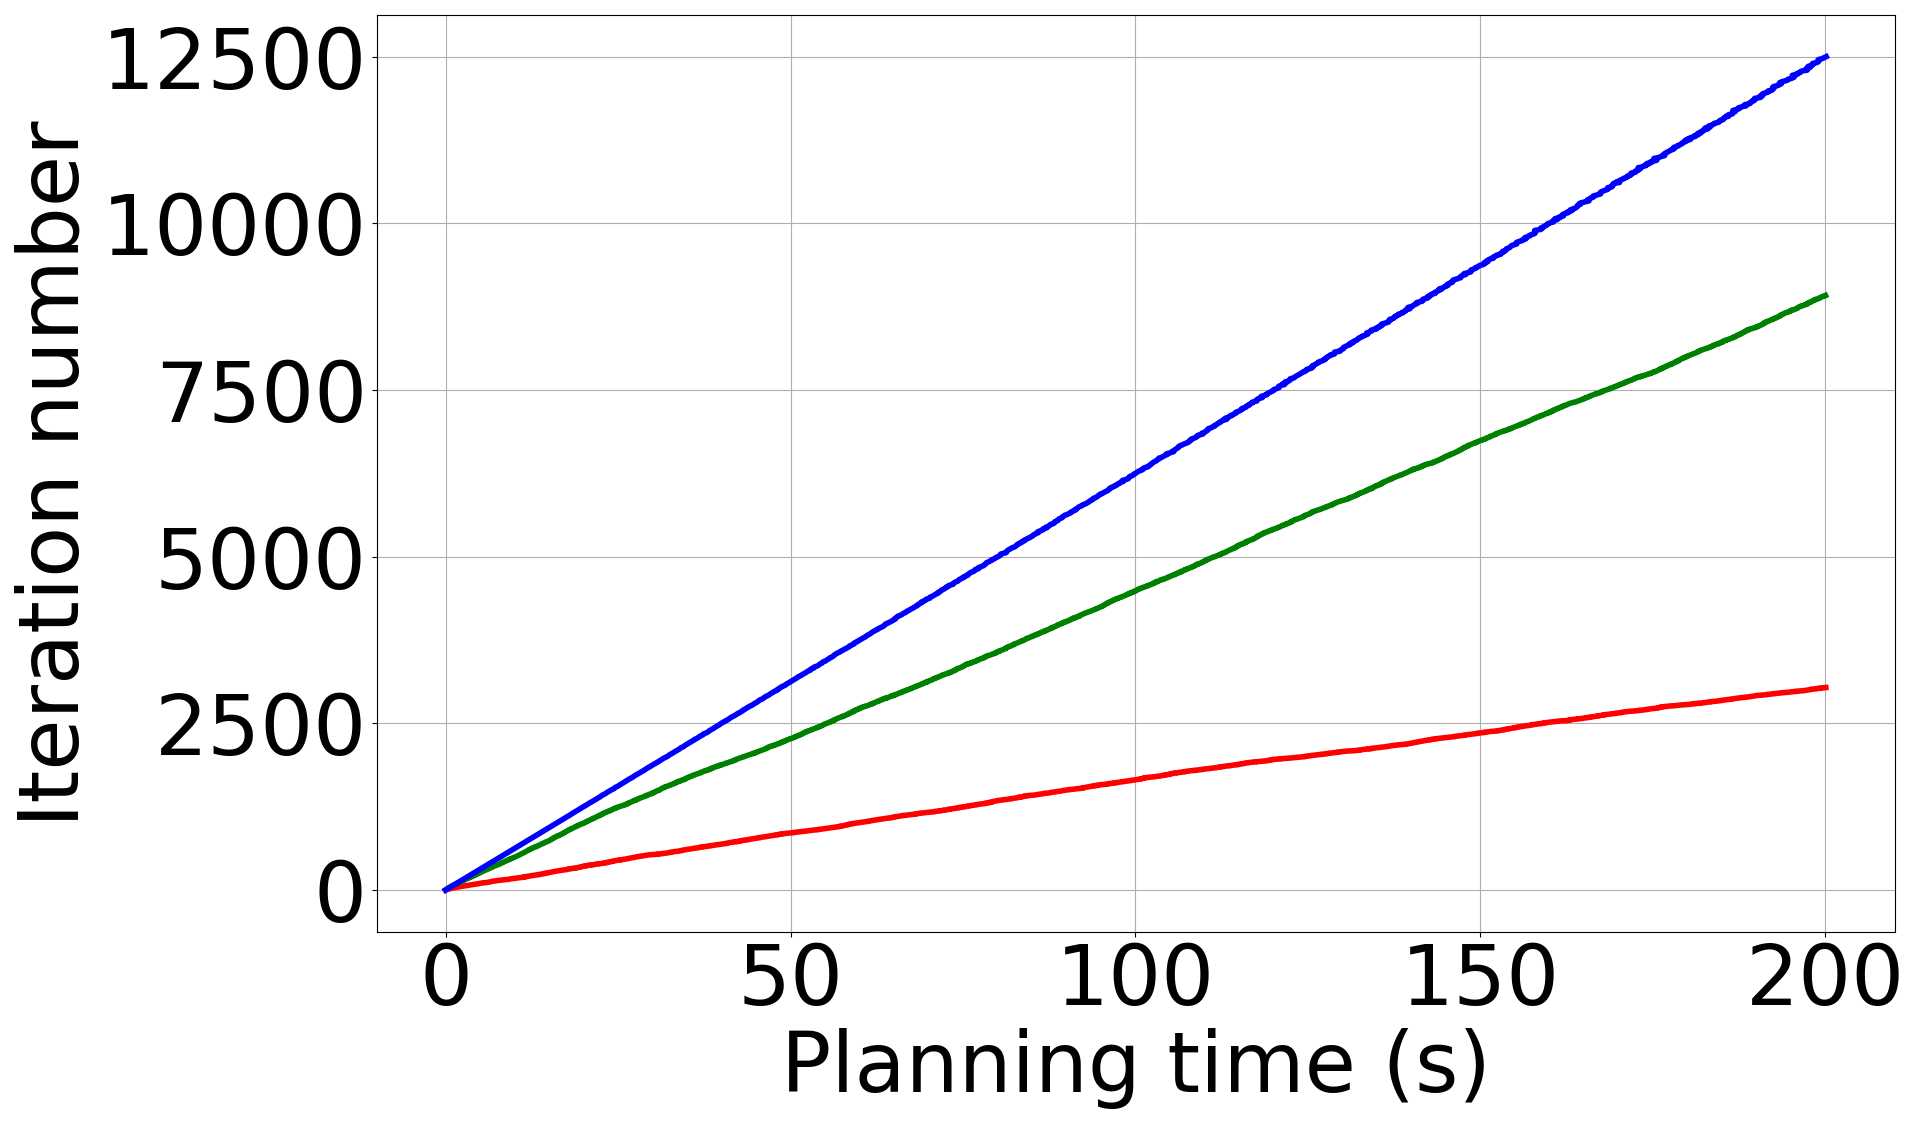
\includegraphics[width=0.4\linewidth]{figures/robust_accurate/iterations_RRT_new.png} }}%
    \subfloat[\centering RRT$^*$]{{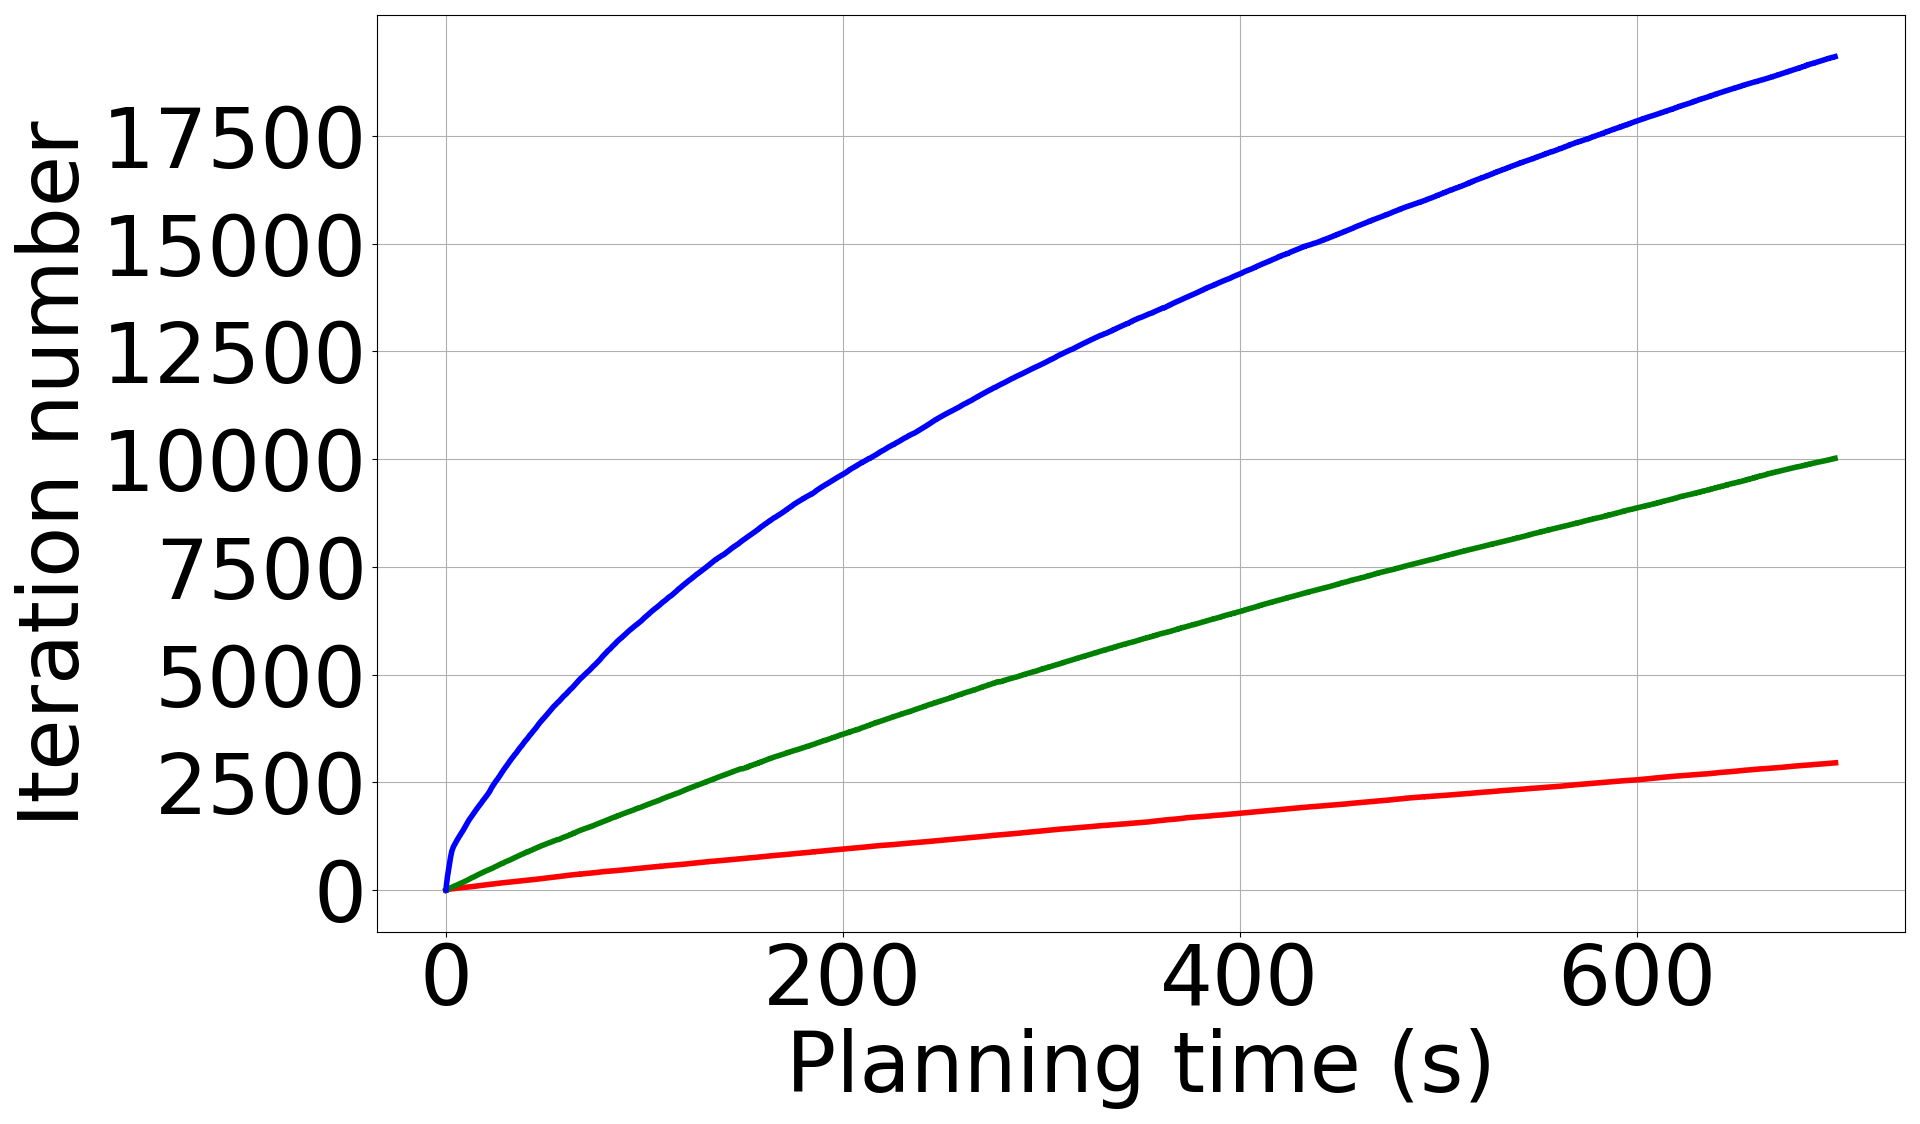
\includegraphics[width=0.4\linewidth]{figures/robust_accurate/iterations_RRTstar_new.png} }}%
    \caption{Number of (a) RRT / (b) RRT$^*$ iterations as a function of planning time in an obstacle-free environment using the standard (non-robust) RRT/RRT$^*$ implementation (blue), compared to \myglsentry{deepsamp} variants that leverage the GRU-based tube prediction (green) or the \myglsentry{samp} variants (see Chapter~\ref{chap:samp}) (red), that solve the entire set of \myglsentry{odes}.}%
    \label{fig: NNTime}%
\end{figure}

\begin{figure} [htp]
    \centering
    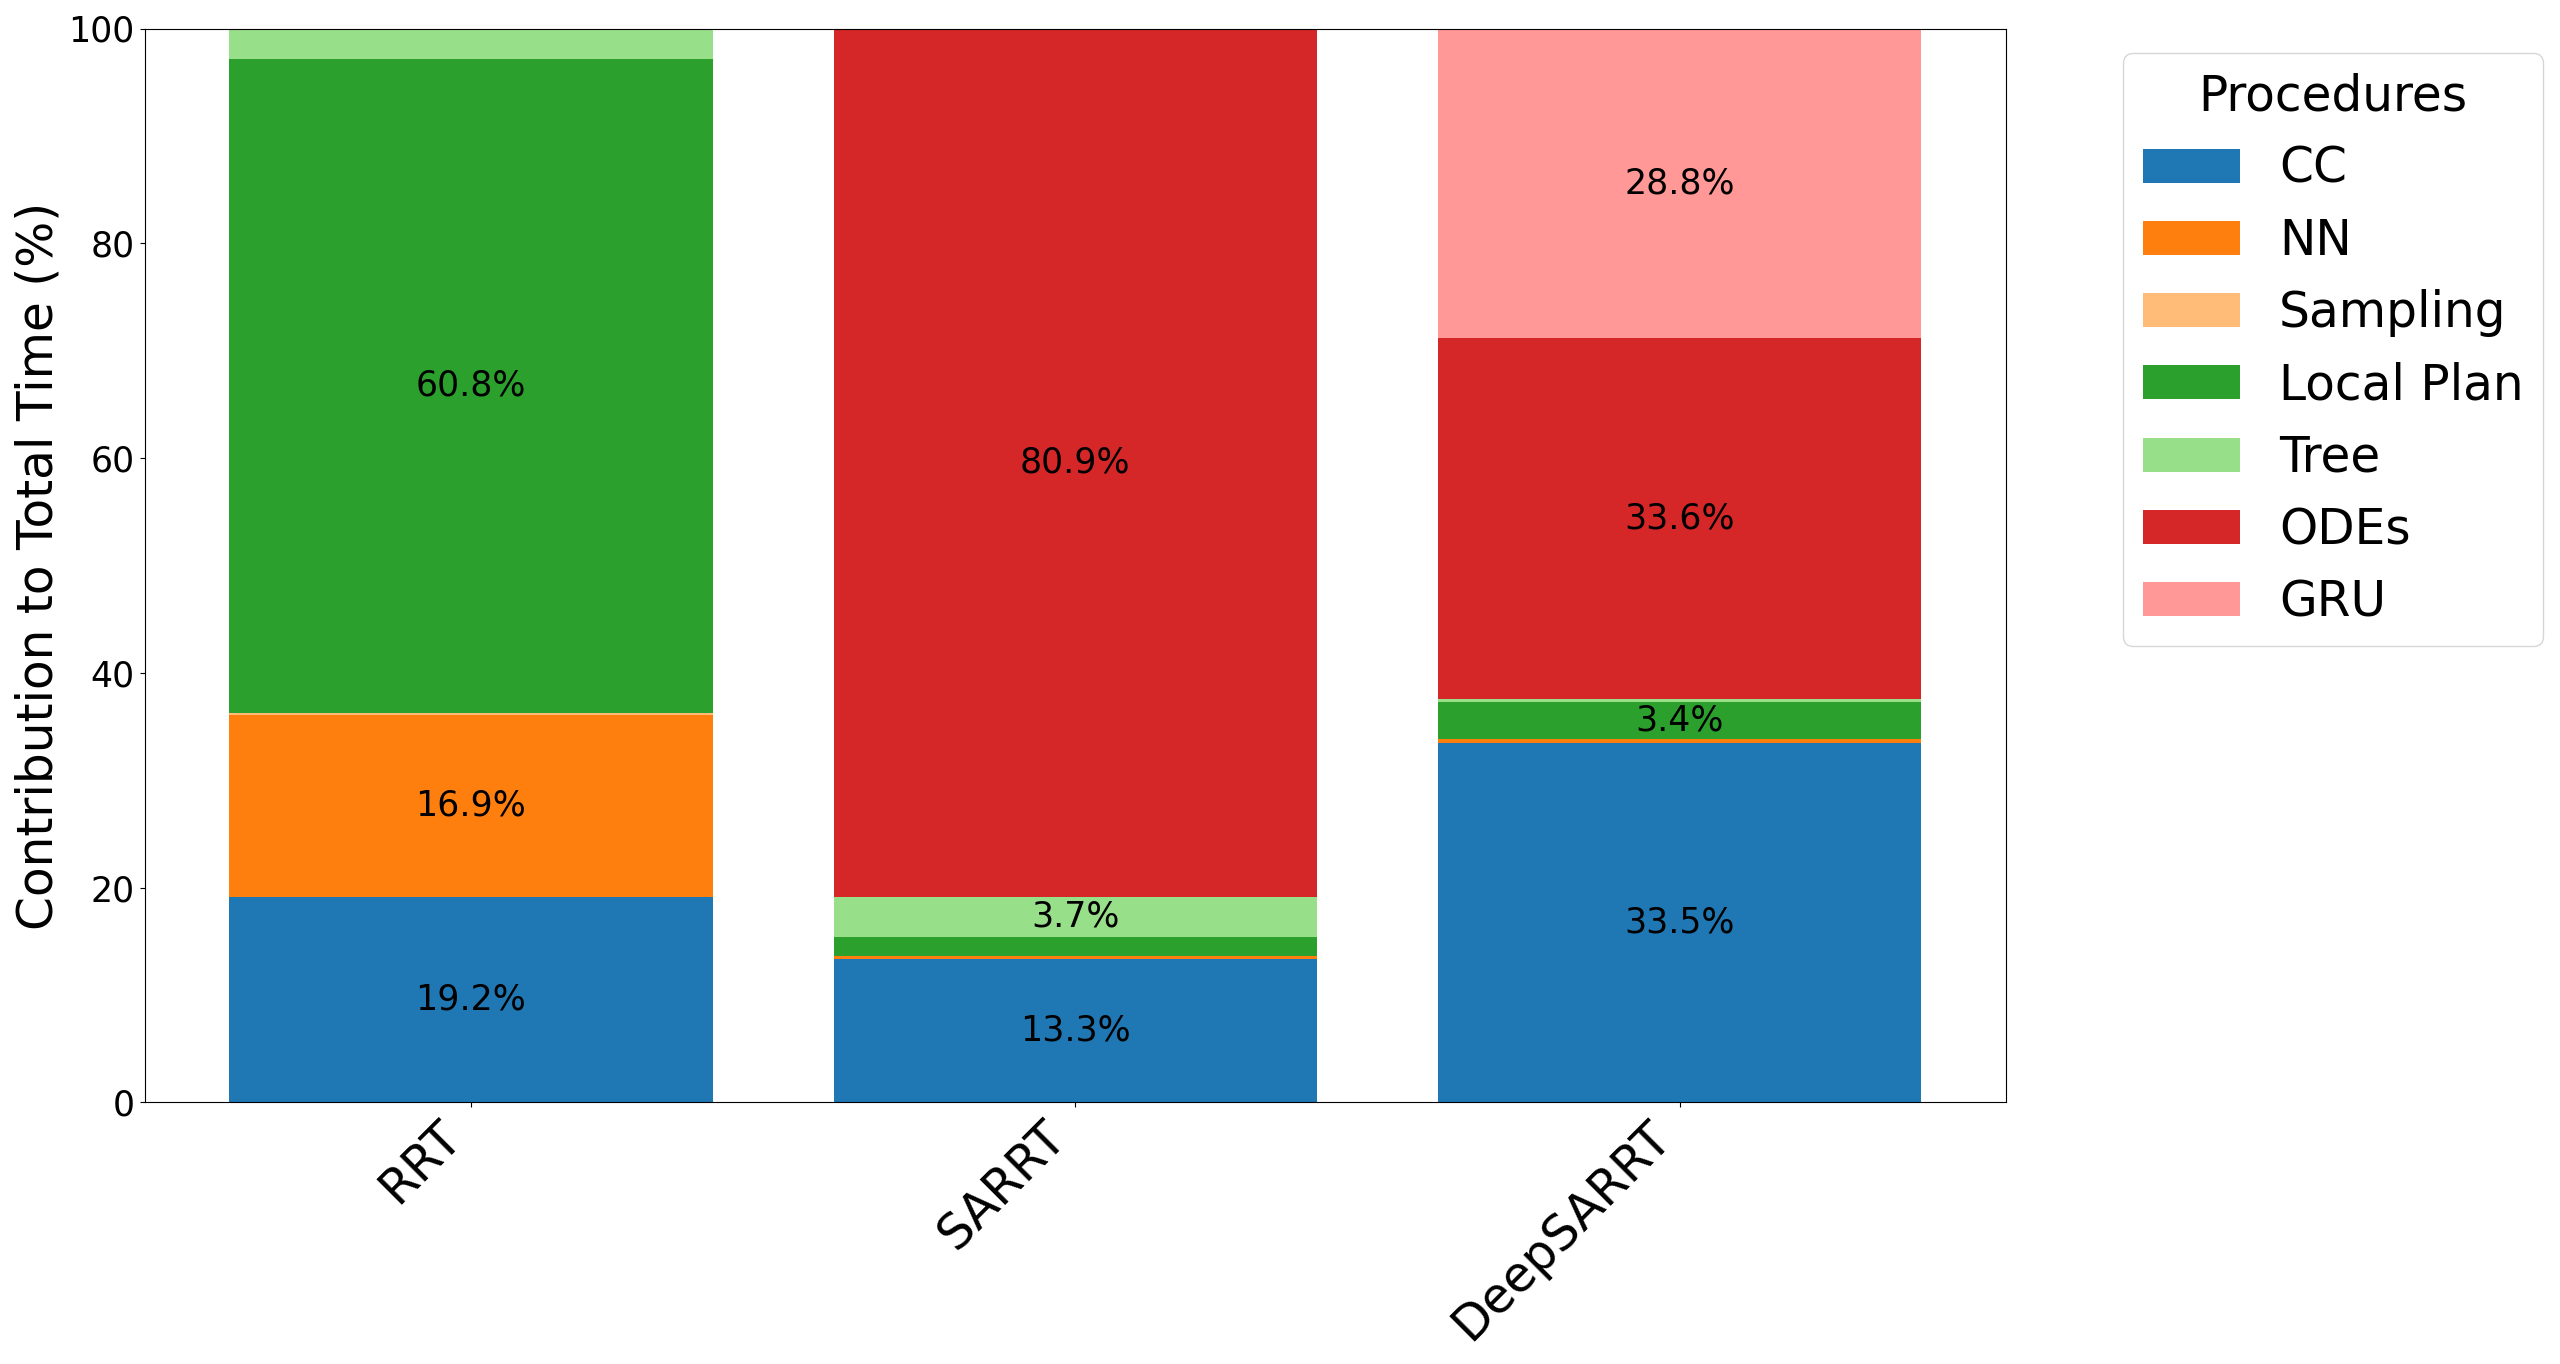
\includegraphics[width=0.9\linewidth]{figures/robust_accurate/profiling_rrt.png}%
    \\
    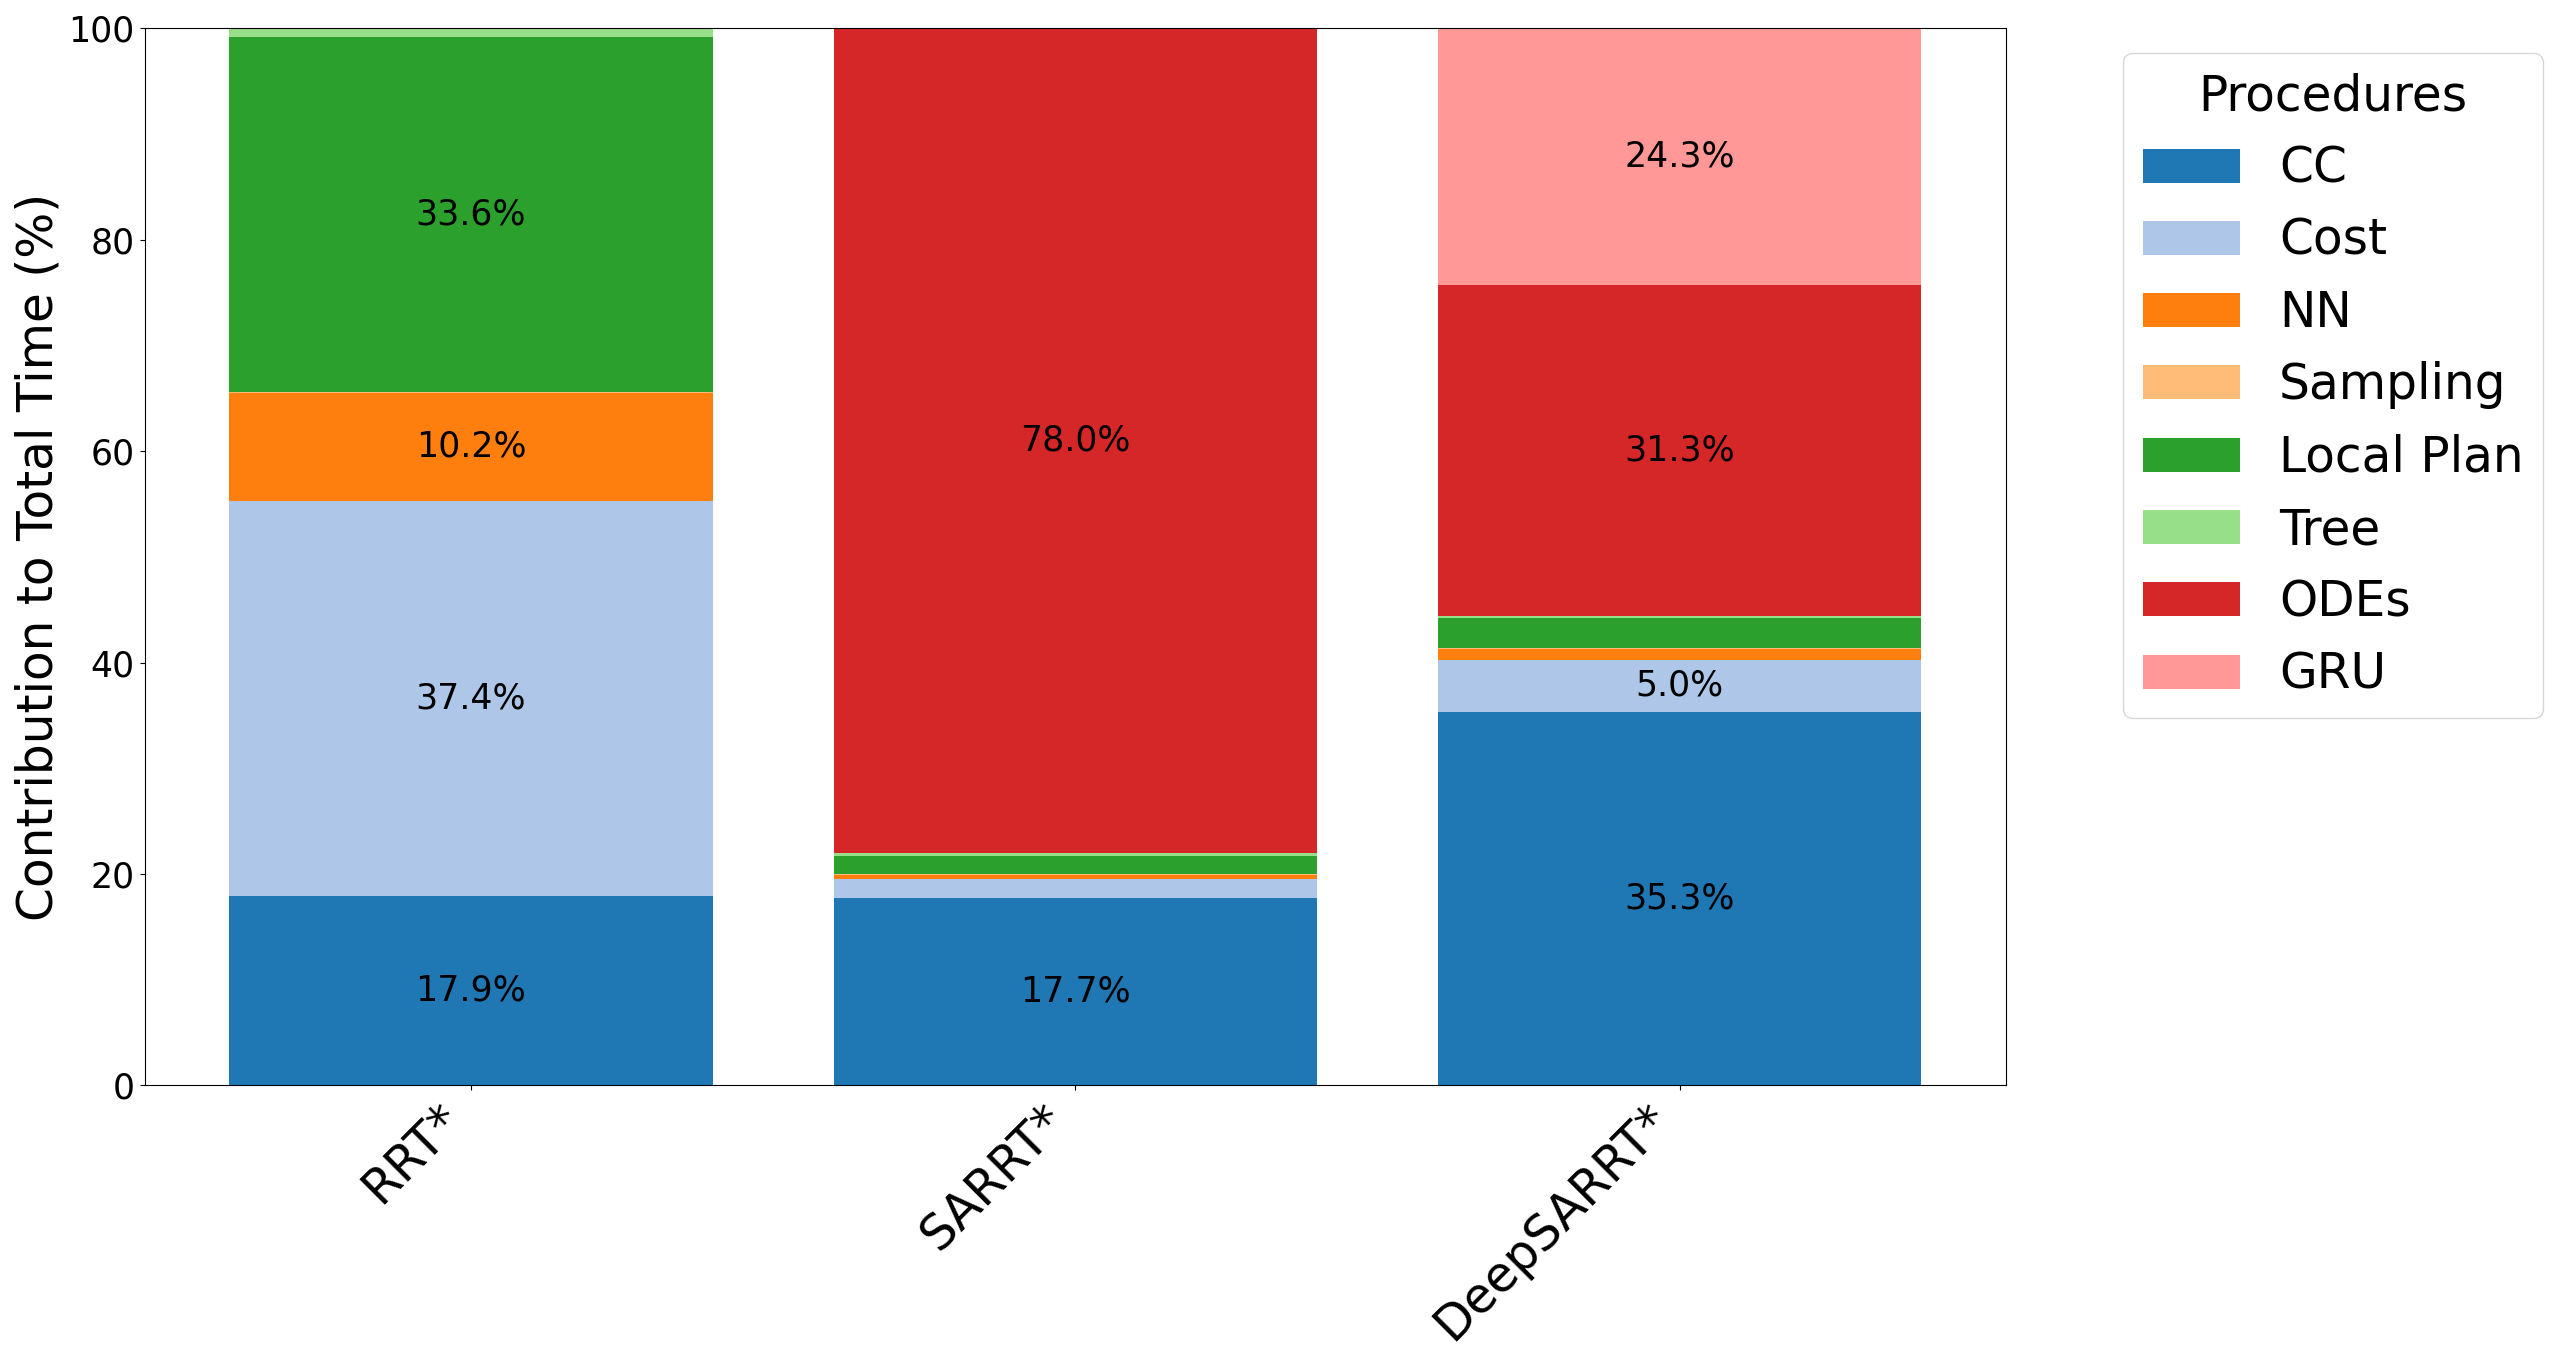
\includegraphics[width=0.9\linewidth]{figures/robust_accurate/profiling_rrtstar.png}%
    \caption{Profiling comparison between vanilla planners, \myglsentry{deepsamp} variants and \myglsentry{samp} variants, illustrating the contributions of various procedures to the total planning time over 1.000 iterations in a free space environment.}%
    \label{fig:NNProfiling}%
\end{figure}

Figure~\ref{fig: NNTime} shows the significant performance improvement of using this learning-based prediction within a sampling-based tree planner for checking the robustness of the local tree expansions (see Algorithm~\ref{alg:ExtensionExample}), against the \myglsentry{samp} variants that solve the entire set of \myglsentry{odes} (see Chapter~\ref{chap:samp}).  
Results provided for RRT and its RRT* near time-optimal variant compare the number of iterations of the main loop of the algorithm as a function of computing time in an obstacle-free environment, showing in both cases a significant time gain thanks to the proposed learning method compared with integrating the entire set of \myglsentry{odes}.
Note that in the case of RRT, this time gain is constant ($3$ times faster) because the expansion benefits from the neural network only once per iteration.
In the case of RRT*, the denser the tree, the more robust collision tests are required for the rewiring connection phase. 
Therefore, much more time is saved when using the learning method. 
The gain on the planning time can reach more than one order of magnitude for problems requiring a significant amount of iterations.

This time saving is also illustrated by Figure~\ref{fig:NNProfiling}, that shows for both asymptotically optimal and non-optimal sensitivity-aware variants, the contribution of solving the \myglsentry{odes} or performing GRU predictions to the total planning time on 1.000 algorithms iterations.
Note that the \myglsentry{rrtstar} and its sensitivity-aware variants optimize the trajectory length.
The sensitivity is then only used to enforce robust constraints.
The results show that the combination of solving solely the system dynamic and performing GRU predictions is less costly than solving the entire \myglsentry{odes} set.
Furthermore, one can note that in all sensitivity-aware variants, the contribution of the collision checking is overall higher than in their standard counterparts.

Finally, note that the predictions are only valid for the parameter maximum range $\delta\p$ chosen during the generation of the training set, and that the model is trained for given values of the controller gains.

%%%%%%%%%%%%%%%%%%%%%%%%%%%%%%%%%%%%%%%%%%%%%%%%%%%%%%%%%%%%%%%%%%%%%%%%%%%%%%%%%%%%%%%%%%%%%%%%%%%%
\subsection{Robust motion planning via deep learning} \label{sec:RobustPlanSimu}

The efficiency and robustness of the DeepSARRT planner (see Section~\ref{sec:RSAMP}) are demonstrated through comparative simulation results against a standard (non-robust) RRT, RandUp-RRT~\cite{cRandUpRRT}, the SARRT variant solving the full set of \myglsentry{odes} as detailed in Chapter~\ref{chap:samp}, and LazySARRT, an RRT implementation of \myglsentry{lazysamp} (see Chapter~\ref{chap:samp}).
The RandUp-RRT has been implemented with 20 ``RandUP particles'' to approximate the reachable set, and no $\epsilon$-padding is used.
The padding value is a user parameter that is difficult to find. 
Choosing the wrong padding value can result in set estimations that are too conservative. 
Therefore, it is set to zero in this thesis as in some experiments of~\cite{cRandUpRRT}.
The LazySARRT performs robust feasibility tests only when a solution is found, disconnecting and reconnecting the tree if necessary via a RobustReconnect procedure, as shown in Algorithm~\ref{alg:LazySARRT*}. 
This procedure  maintains and updates a set of non-robust connections for each node in the tree. In the case of \myglsentry{lazysarrt*}, the RobustReconnect procedure also ensures tree optimality. 
Consequently, all nodes, starting from the first non-robust node, are disconnected and reconnected optimally.
In contrast, the LazySARRT does not consider optimality. 
Therefore, children nodes are disconnected from their parent and reconnected to the tree only if their parent is deleted.
This strategy significantly reduces the number of reconnection attempts.

A \myglsentry{deepsamp} variant of the \myglsentry{rrtstar}, denoted DeepSARRT*, is compared to the classic non-robust RRT* and the two variants proposed in Chapter~\ref{chap:samp}, SARRT* and LazySARRT*. 
These optimal planners compute near time-optimal trajectories and ran until the solution cost converged below a threshold of 15 seconds. 
The RandUp-RRT was excluded from this comparison, as no optimal version of the algorithm exists.

The comparison is based on the several planenrs planning time and success rate on the scenario depicted in Figure~\ref{fig: fig1robust}, using an Intel i9 CPU@2.6GHz and a RTX A3000 GPU for the GRU predictions.
Table~\ref{tab:Robust window} and Table~\ref{tab:Robust window star} show comparative results for optimal and non-optimal planners, averaged for each planner over 20 trajectories and 30 simulations with uncertain parameters uniformly sampled in the range $\delta\p$ presented in Section~\ref{sec:quad_setup}. 
Note that since the sensitivity-based uncertainty tubes are valid for uncertain parameters contained within the uncertain parameter ellipsoid (see Section~\ref{sec:tubes}), the sampled vector of uncertain parameters is projected onto the ellipsoid hull when necessary.

First note that RandUp-RRT, SARRT, LazySARRT and DeepSARRT have a much stronger robustness than standard non-robust RRT. 
All SARRT, LazySARRT and DeepSARRT have a success rate of 100\% compared to 99.2\% for RandUp-RRT. 
Indeed, as mentioned in~\cite{cRandUpRRT, cRandUP}, the computation of a conservative reachable set requires some additional padding step, which is here set to zero as mentioned earlier.

Also note the higher efficiency of DeepSARRT which only uses one prediction per iteration whereas RandUp-RRT needs to perform a propagation per particle, yielding to a longer planning time. 
Additionally, DeepSARRT demonstrates greater efficiency compared to its SARRT counterparts, with three times the time savings, as highlighted in Section~\ref{sec:NNresult}.
As for LazySARRT, it does not build a robust tree like DeepSARRT. 
Instead, it only robustly checks the final solution, causing frequent disconnections and re-connections of non-robust nodes, which results in a higher planning time.
RRT, which does not account for robustness, remains faster but with a significantly lower success rate. 
Similar results are observed on the optimal versions. 
One can note the efficiency of the DeepSARRT* that reach approximately one order of magnitude time gain (mentioned in Section~\ref{sec:NNresult}) compared to its \myglsentry{sarrt*} counterparts. 
An example of trajectories planned by RRT* and a robust version DeepSARRT* optimizing the trajectory duration, and their associated simulations, is illustrated in Figure~\ref{fig: simu window}.
It shows the effective robustness of the proposed algorithm as illustrated by the higher success rate indicated in Table~\ref{tab:Robust window} and Table~\ref{tab:Robust window star}.

\begin{table*}[t!]
    \centering
    \begin{tabular}{l|lllll|}
    \cline{2-6} & \multicolumn{5}{c|}{Basic Planners} \\ \cline{2-6} 
        & \multicolumn{1}{c|}{RRT} & \multicolumn{1}{c|}{RandUp-RRT} & \multicolumn{1}{c|}{SARRT} & \multicolumn{1}{c|}{LazySARRT} & \multicolumn{1}{c|}{DeepSARRT} \\ \hline
    \multicolumn{1}{|c|}{Success (\%)} & \multicolumn{1}{c|}{61.8}   & \multicolumn{1}{c|}{99.2} & \multicolumn{1}{c|}{\textbf{100.0}}  &   \multicolumn{1}{c|}{\textbf{100.0}}  & \multicolumn{1}{c|}{\textbf{100.0}}\\ \hline
    \multicolumn{1}{|c|}{Plan time (s)} & \multicolumn{1}{c|}{\textbf{7.1} $\pm$ 7.6}  & \multicolumn{1}{c|}{57.8 $\pm$ 49.1}  & \multicolumn{1}{c|}{ 78.5 $\pm$ 55.1} & \multicolumn{1}{c|}{45.6 $\pm$ 33.4} &   \multicolumn{1}{c|}{ 22.3 $\pm$ 15.8} \\ \hline
    \end{tabular}

    \caption{
    \label{tab:Robust window}
    Quadrotor application: Average planning time and robust feasibility success rates of the simulated motions planned using standard non-robust RRT, RandUP-RRT, the SARRT variant (see Chapter~\ref{chap:samp}), LazySARRT (see Chapter~\ref{chap:samp}), and DeepSARRT.
    The results are averaged over 20 plans and 30 simulations per plan.}
\end{table*}
\begin{table*}[htp]
    \centering
    \begin{tabular}{l|llll|}
    \cline{2-5} & \multicolumn{4}{c|}{Optimal Planners} \\ \cline{2-5} 
        & \multicolumn{1}{c|}{RRT*} & \multicolumn{1}{c|}{SARRT*} & \multicolumn{1}{c|}{LazySARRT*} & \multicolumn{1}{c|}{DeepSARRT*} \\ \hline
    \multicolumn{1}{|c|}{Success (\%)} & \multicolumn{1}{c|}{56.5}  &  \multicolumn{1}{c|}{\textbf{100.0}} &  \multicolumn{1}{c|}{\textbf{100.0}}  &  \multicolumn{1}{c|}{\textbf{100.0}}   \\ \hline
    \multicolumn{1}{|c|}{Plan time (s)} & \multicolumn{1}{c|}{\textbf{308.7} $\pm$ 235.7}  &   \multicolumn{1}{c|}{ 5459.5 $\pm$ 817.5} &   \multicolumn{1}{c|}{834.3 $\pm$ 380.0}  &  \multicolumn{1}{c|}{584.3 $\pm$ 394.7}    \\ \hline
    \end{tabular}

    \caption{
    \label{tab:Robust window star}
    Average planning time and robust feasibility success rates of the simulated motions planned using standard non-robust RRT*, \myglsentry{sarrt*} (see Chapter~\ref{chap:samp}), \myglsentry{lazysarrt*} (see Chapter~\ref{chap:samp}) and the DeepSARRT* variant, all of them optimizing trajectory length.
    The results are averaged over 20 plans and 30 simulations per plan, except for the \myglsentry{sarrt*}, which values are averaged over 3 runs and 30 rollouts per plan due to long planning time.}
\end{table*}

\begin{figure} [htp]
    \centering
    \subfloat[\centering RRT*]{{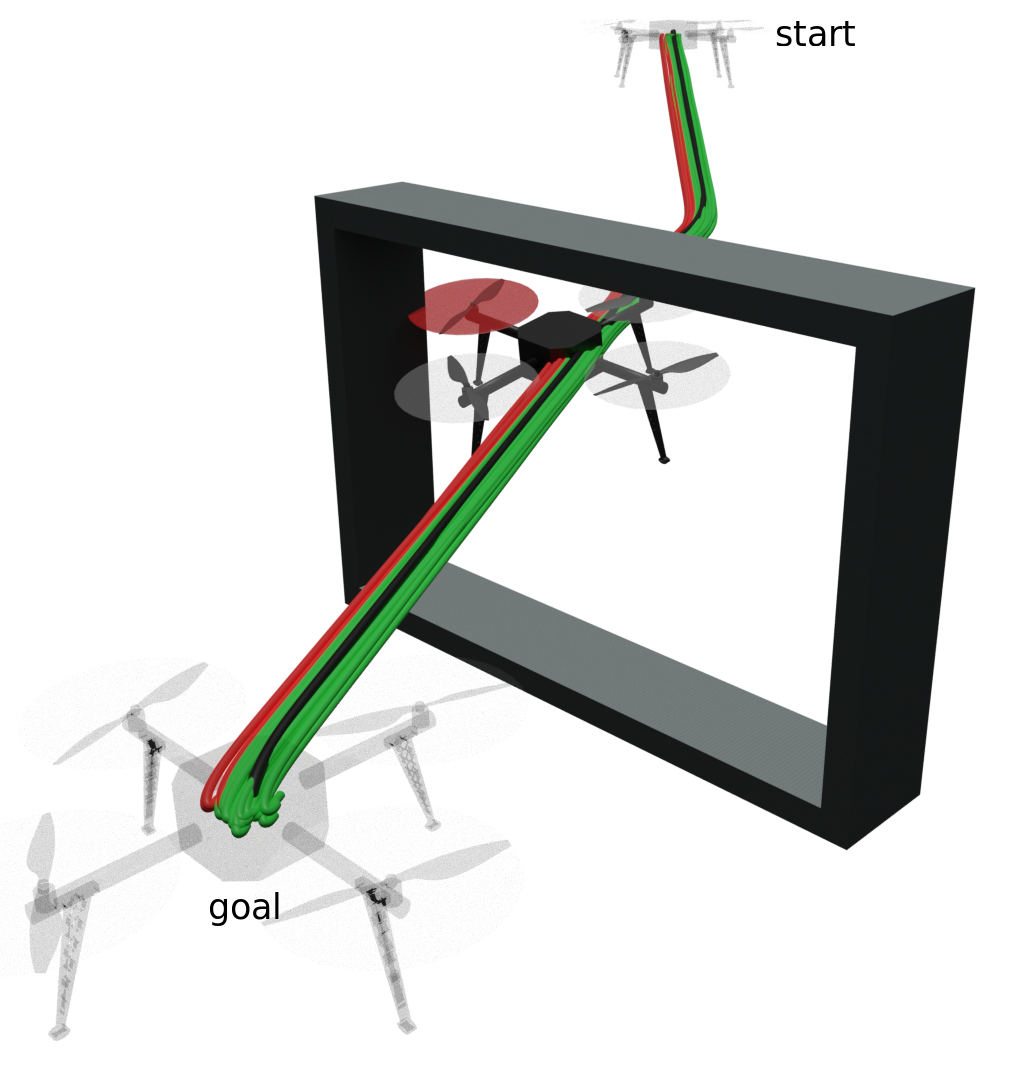
\includegraphics[width=0.4\linewidth]{figures/robust_accurate/simu_RRTstar_notube.png} }}%
    \subfloat[\centering R-SARRT*]{{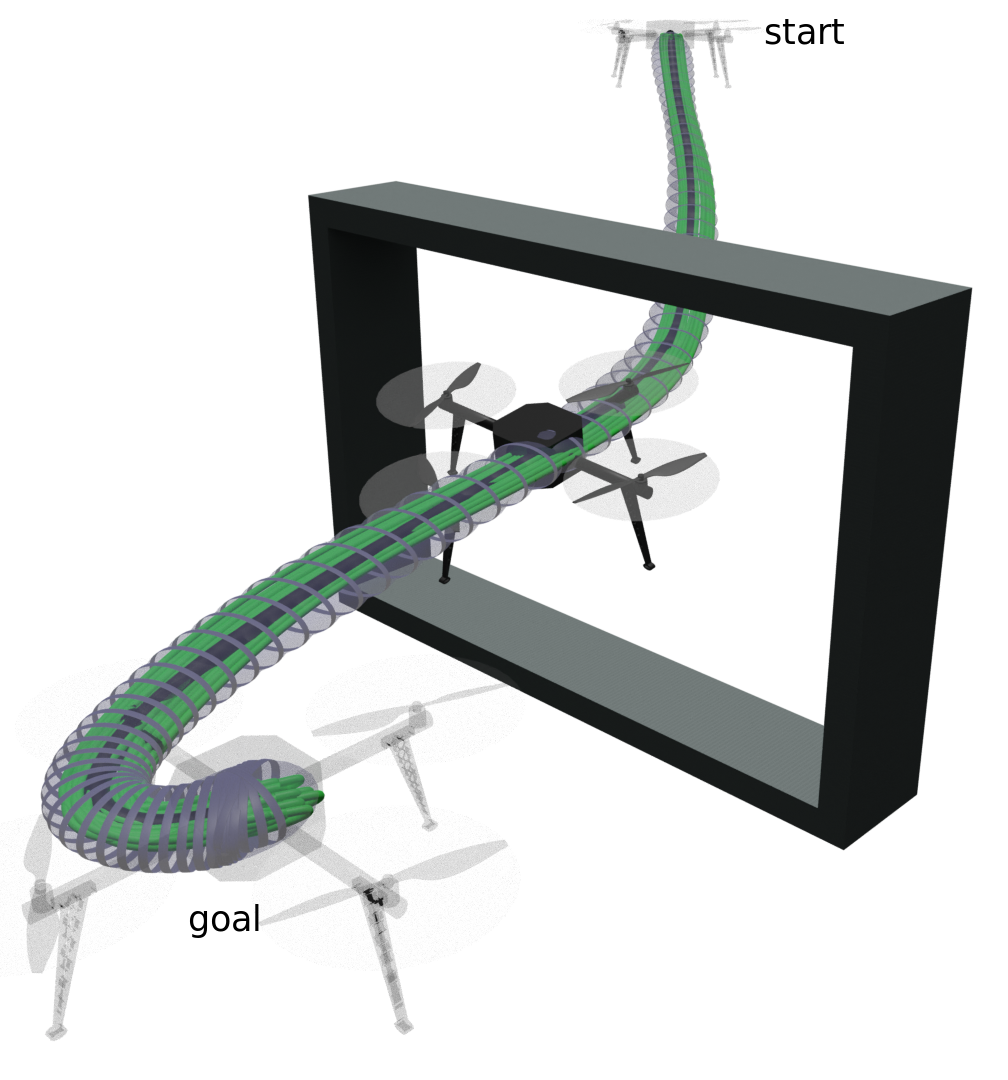
\includegraphics[width=0.4\linewidth]{figures/robust_accurate/simu_SARRTstar.png} }}%
    \caption{Planned trajectory (black) produced by a (a) RRT* and (b) DeepSARRT*. 
    Simulated trajectories under uncertainty are displayed in green in the case of success, and in red in the case of a crash.}%
    \label{fig: simu window}%
\end{figure}

%%%%%%%%%%%%%%%%%%%%%%%%%%%%%%%%%%%%%%%%%%%%%%%%%%%%%%%%%%%%%%%%%%%%%%%%%%%%%%%%%%%%%%%%%%%%%%%%%%%%
\subsection{Robust local accuracy optimization} \label{sec:AccOptSimu}

This section provides a comparison of the robust sensitivity-aware local optimizers introduced in Section~\ref{sec:AOptim}. 
The evaluation focuses on their computation time and resulting costs, using an initial trajectory as the optimization variable.
The objective is to identify the most suitable optimizer for the accuracy optimization stage required for the experimental scenario outlined in Section~\ref{sec:AccOptExp}.

All algorithms are tested on three different environments and stop when a cost convergence at 1\% is reached.
The cost function~\eqref{eq: cost} is to be optimized, where the radii of interest are the ones along the $\boldsymbol{x}$, $\boldsymbol{\rho}$ and $\boldsymbol{\omega}$ components of $\boldsymbol{q}$.

Since none of the robust local optimizers guarantee convergence to a robust solution, but do guarantee the preservation of initial robustness, the initial trajectories are planned using the DeepSARRT variant.

\begin{figure} [htp]
    \centering
    \subfloat[\centering Window environment]{{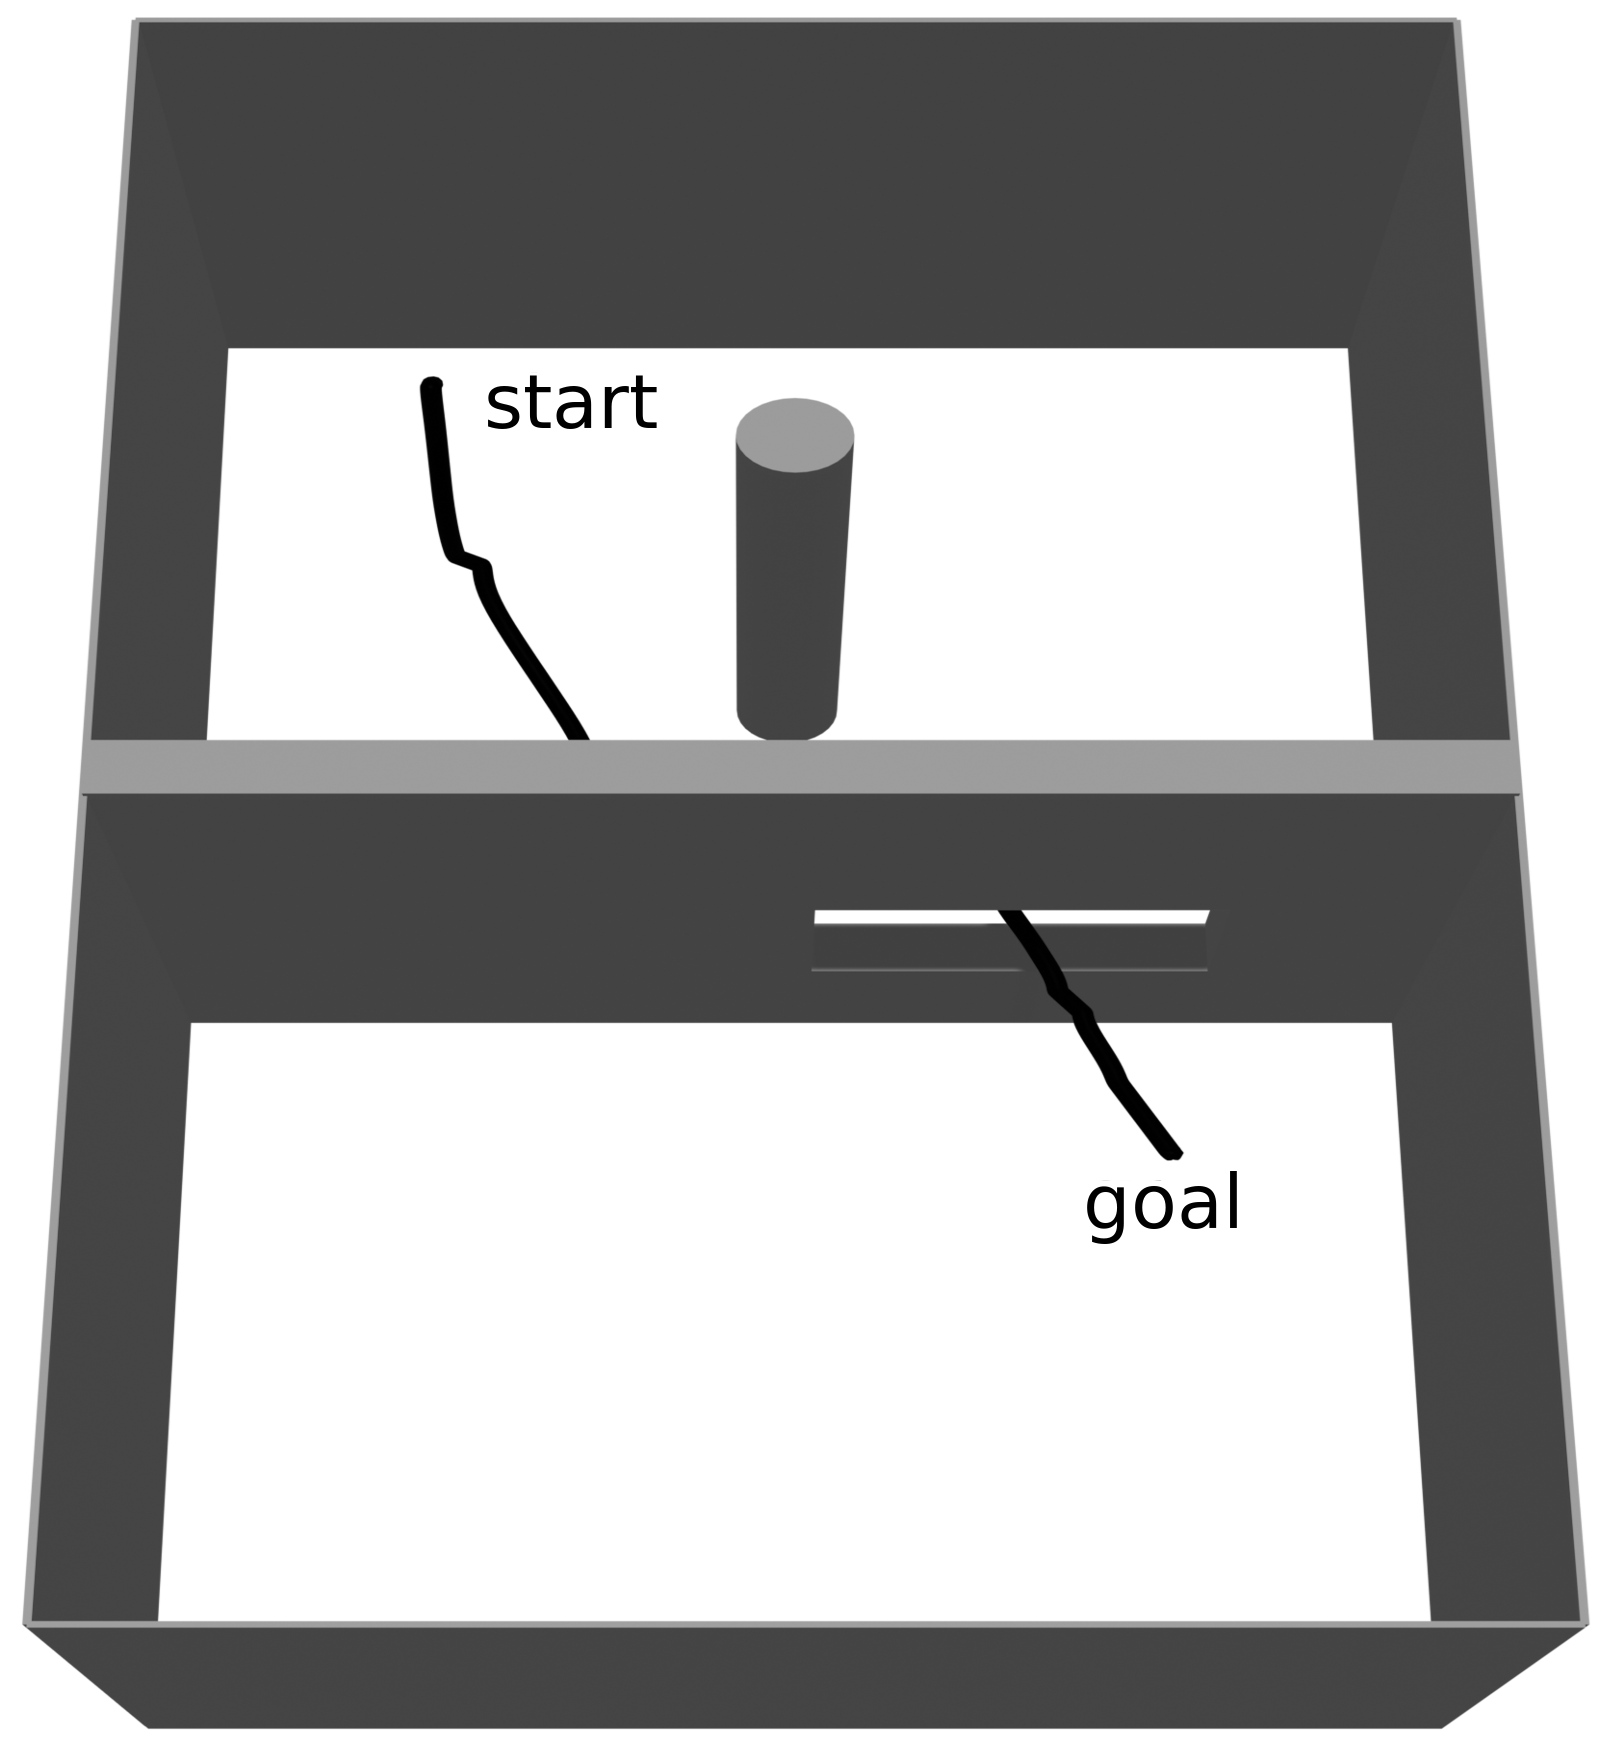
\includegraphics[width=0.4\linewidth]{figures/accuracy/iloveimg-resized/window_pilar.png} }\label{fig:window_pilar}}%
    \subfloat[\centering Corridor environment]{{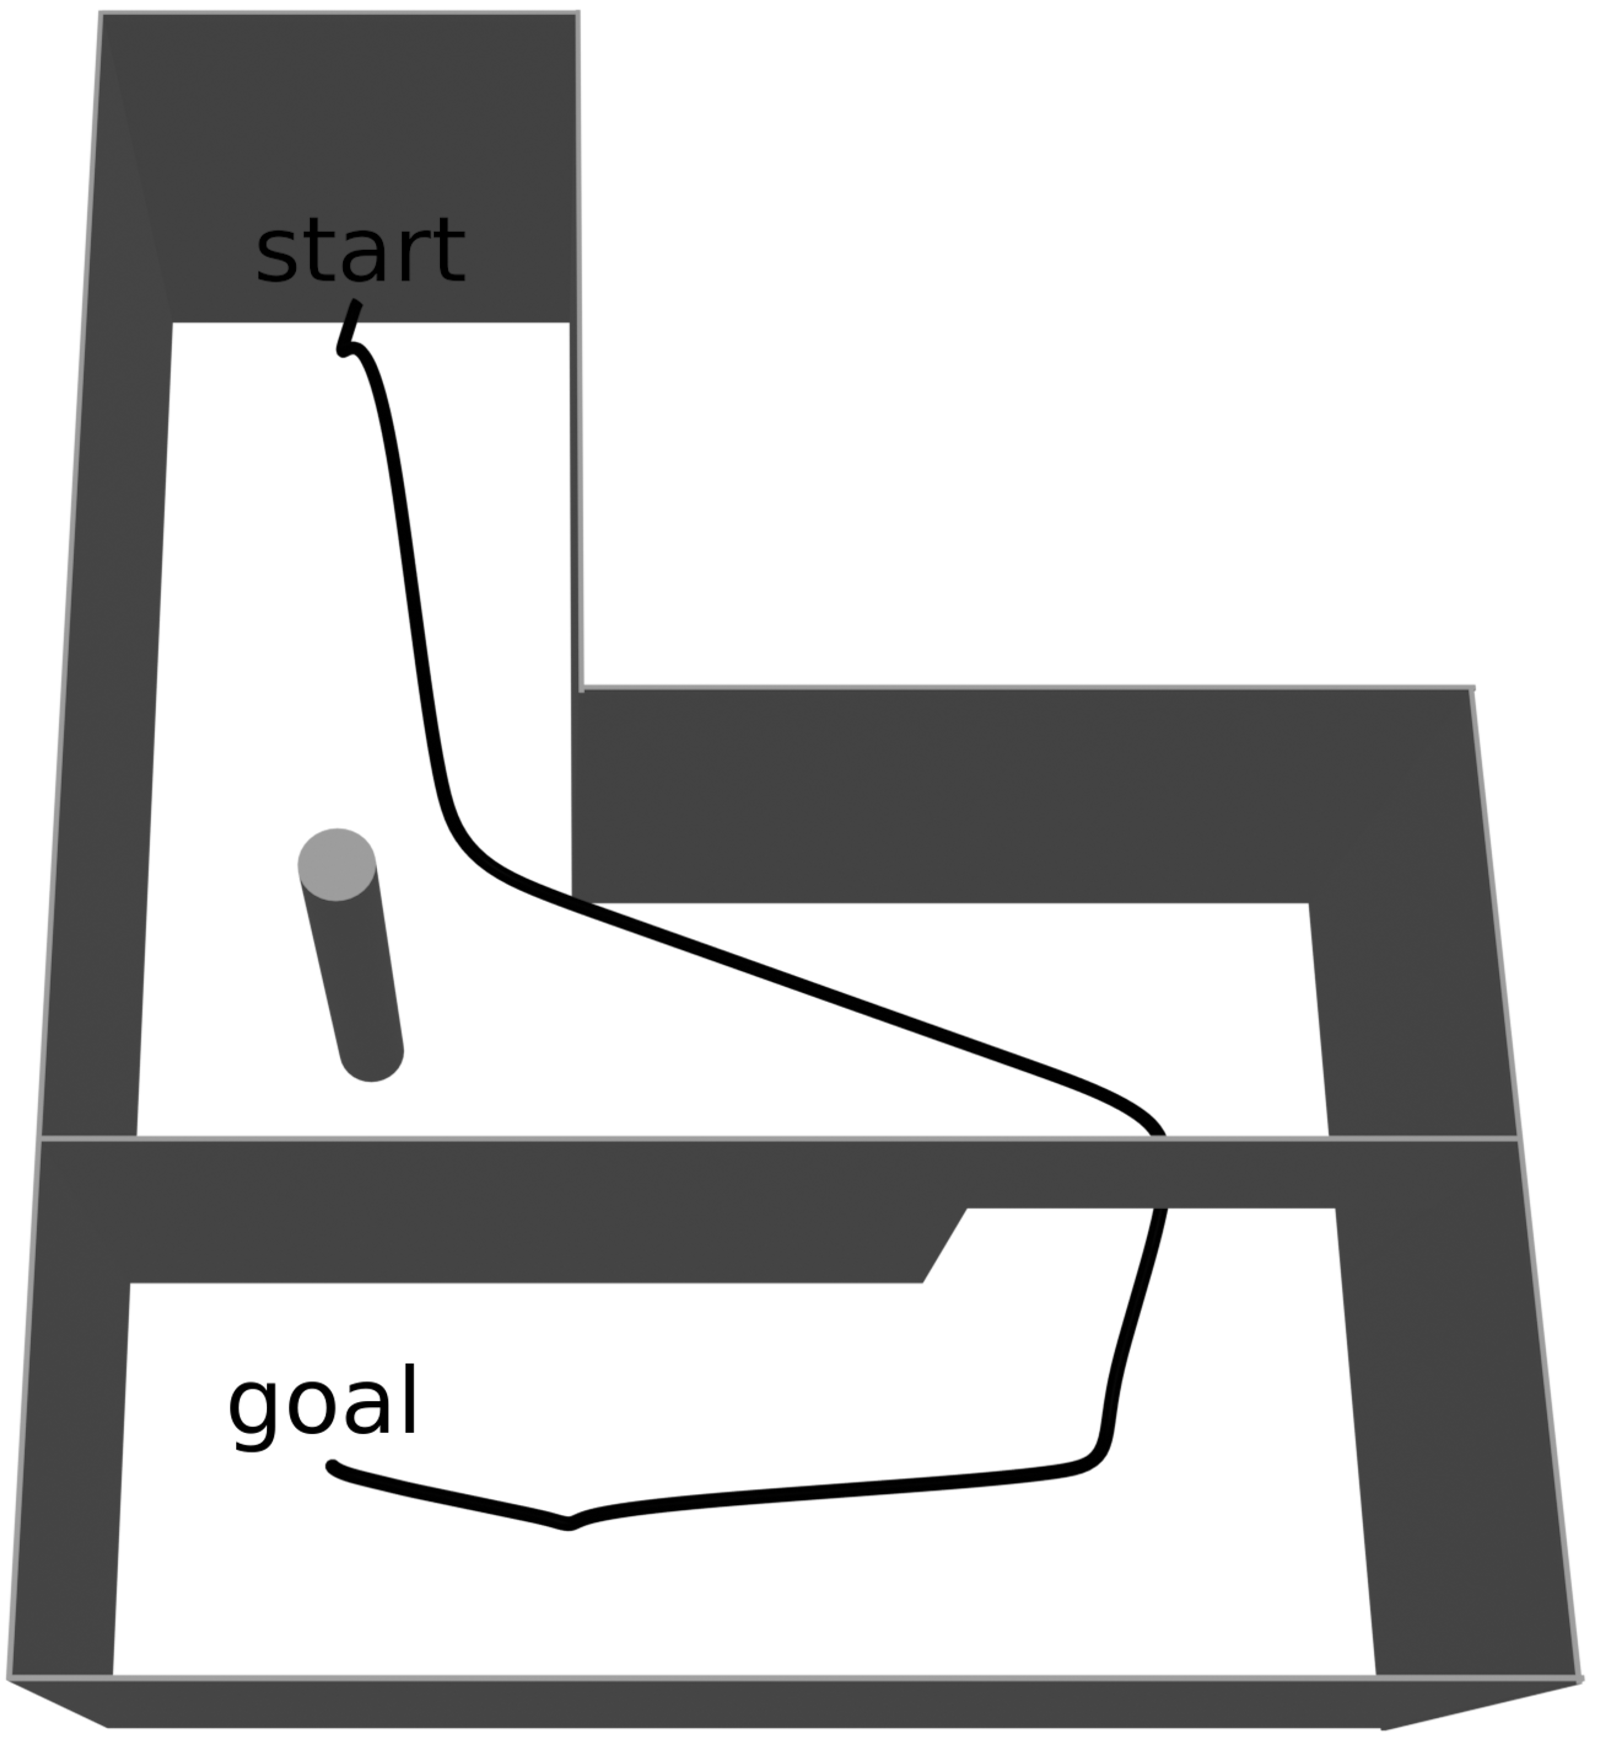
\includegraphics[width=0.4\linewidth]{figures/accuracy/iloveimg-resized/corridor.png} } \label{fig:corridor}}%
    \caption{The two environments considered for the comparison of robust local optimizers, displayed with an initial trajectory guess for the optimization planned by DeepSARRT (black):
    (a) the window environment similar to the one of Section~\ref{sec:RobustPlanSimu} with an additional obstacle, and (b) a narrow corridor environment.}%
\end{figure}

\paragraph{Free space environment}

First, the algorithms are tested in an environment without obstacles to evaluate their ability to escape the local minimum defined by the initial trajectory.
\myglsentry{sastomp} performs 10 rollouts and uses a standard deviation of 0.2 m to generate noisy trajectories.
\myglsentry{saextendedshct} is evaluated with different hyperparameters as follows: $\delta \in \{0.1, \, 0.01\}$ and $K \in \{1, \, 2, \, 3, \, 5, \, 10\}$.
Two different sampling strategies are also tested: a uniform sampling that uses the same radius $\delta$ across all components of the state, and a Gaussian sampling where $\delta$ is used as the standard deviation.

Figure~\ref{fig:acc_empty} provides the optimization results of the four local optimizers in a free space environment.
The \myglsentry{saextendedshct} algorithm is executed using a Gaussian sampling, with $\delta = 0.1$ and $K = 1$, as they are the best hyperparameters find for this scenario according to a grid search that can be found in Appendix~\ref{chap:appendixC}.
First, note how the \myglsentry{cobyla} algorithm remains local in the vicinity of the initial guess.
This behavior suggests the inherent difficulty in linearly approximating the cost function at hand.
Furthermore, note that no standard deviation is observed for \myglsentry{cobyla} denoting the deterministic nature of the algorithm.

Then, one can note that the \myglsentry{sastomp} achieves the best optimization, but with significantly slower convergence compared to both \myglsentry{SAshortcut} and \myglsentry{saextendedshct}.
Finally, the latter two methods achieve convergence within the same planning time, with a better optimization achieved by \myglsentry{saextendedshct} due to its better ability to explore the surrounding of the initial guess.

\begin{figure} [htp]
    \centering
    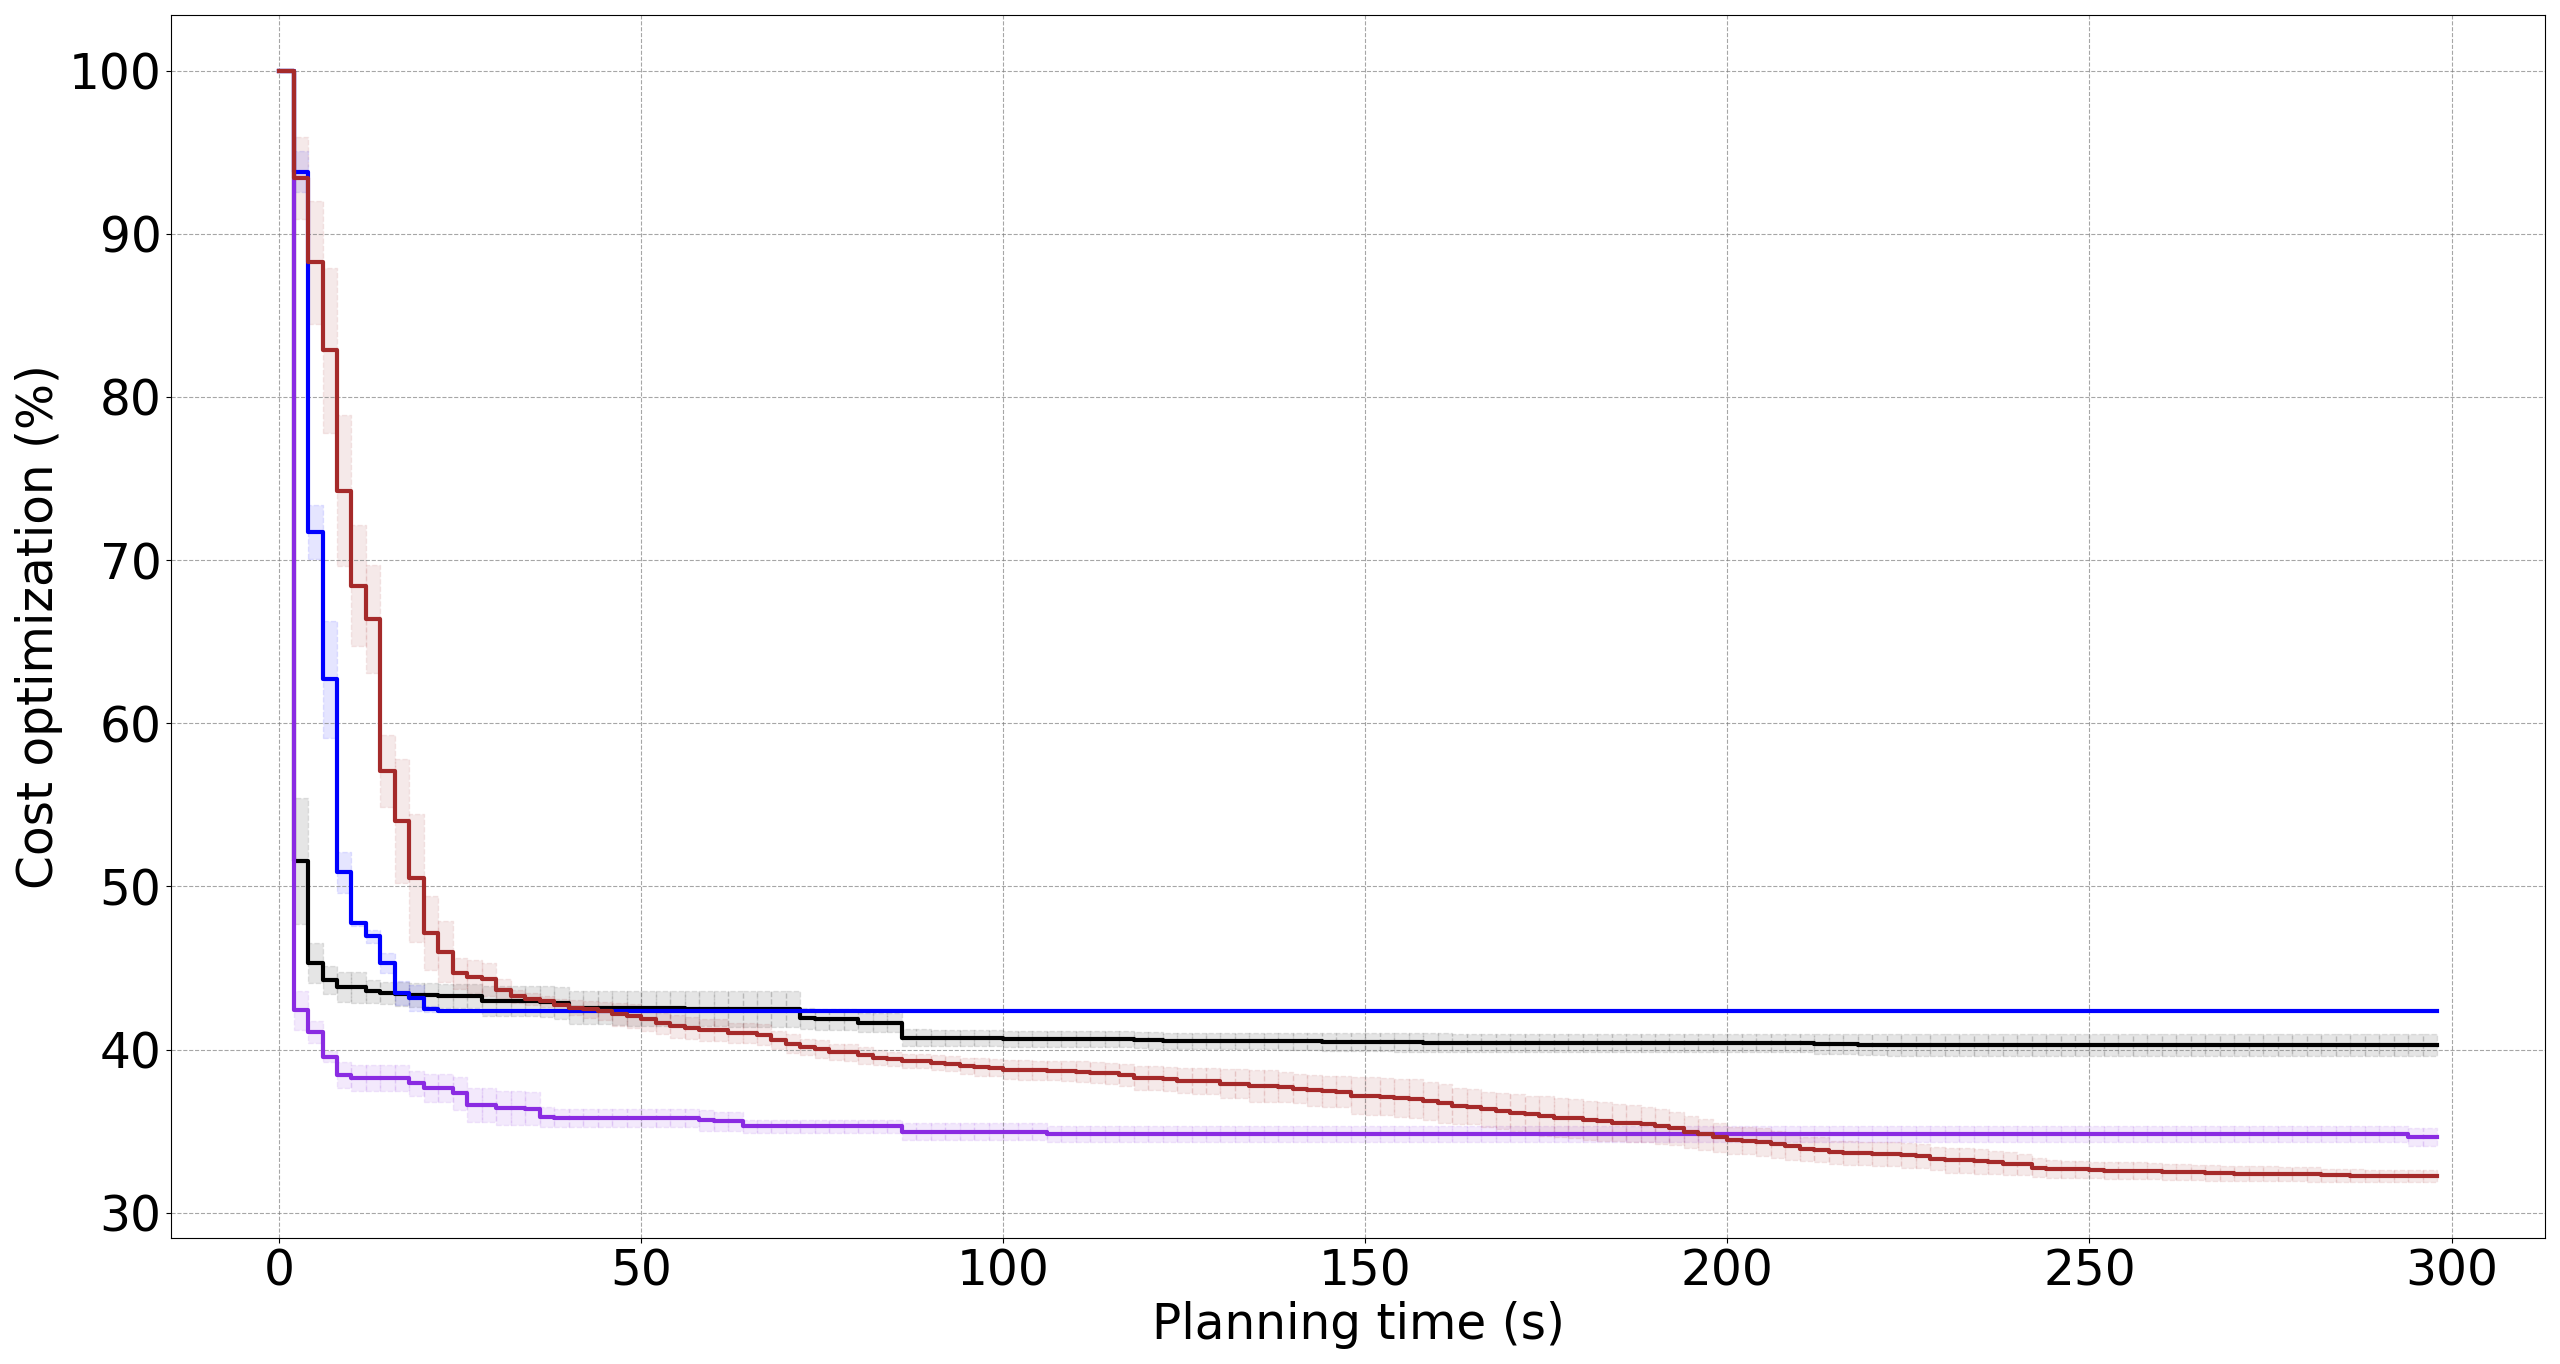
\includegraphics[width=0.9\linewidth]{figures/accuracy/all_methods_empty.png} \\
    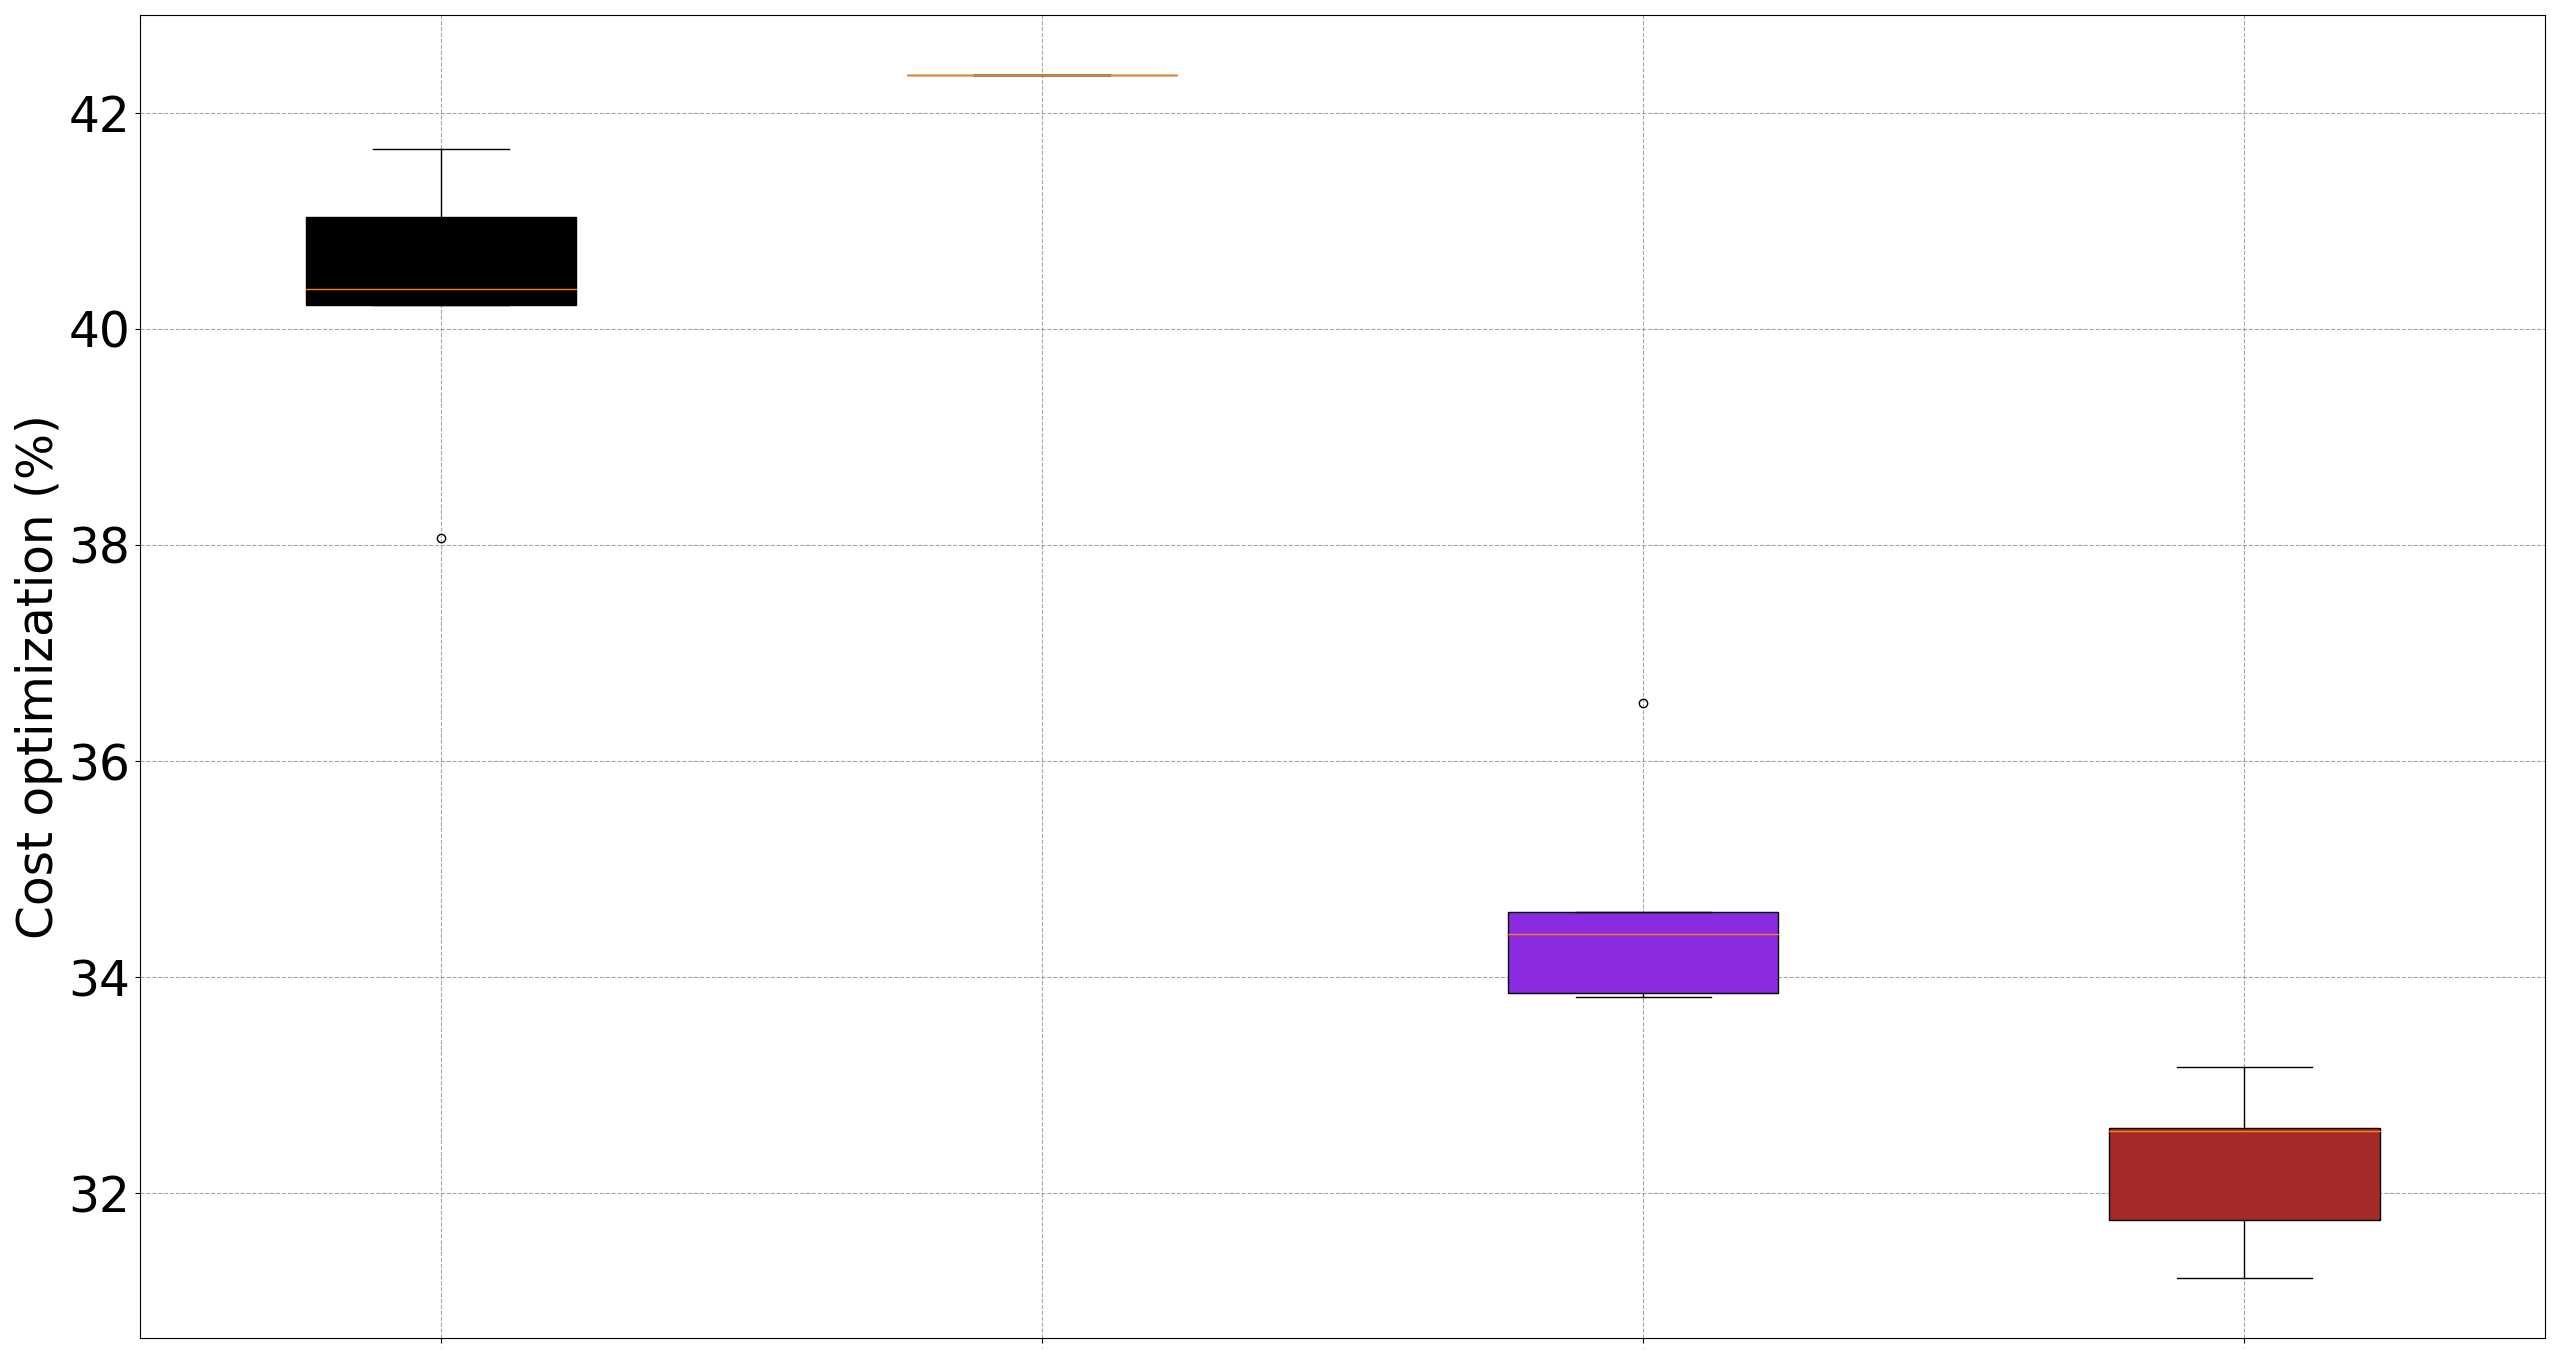
\includegraphics[width=0.9\linewidth]{figures/accuracy/bplot_all_methods_empty.png}
    \caption{Cost optimization results for the four methods outlined in Section~\ref{sec:AOptim}, averaged over 10 plans in a free space environment. 
    The standard deviation is represented as an envelope around the mean curves.
    The \myglsentry{sastomp} is shown in red, \myglsentry{SAshortcut} in black, \myglsentry{saextendedshct} in purple, and \myglsentry{cobyla} in blue.}%
    \label{fig:acc_empty}%
\end{figure}

\paragraph{Window environment}

In order to assess the scalability of the proposed robust optimizer when handling the robust feasibility check (see Section~\ref{sec:robust_CC}), the methods are compared in the environment depicted in Figure~\ref{fig:window_pilar}.
The optimization results are shown in Figure~\ref{fig:acc_window}.
First, note that the \myglsentry{cobyla} algorithm still struggles to explore larger cost areas beyond the vicinity of the initial solution.
Furthermore, the \myglsentry{sastomp} also faces difficulty to efficiently explore the surrounding of the initial trajectory, as denoted by its very slow convergence.
This indicates an inefficient scalability of the algorithm to robust constrained problems.

Both the \myglsentry{SAshortcut} and \myglsentry{saextendedshct} achieve fast convergence with efficient optimization. 
However, while \myglsentry{saextendedshct} outperforms \myglsentry{SAshortcut} in the obstacle-free environment presented above, this is not the case in the presence of obstacles. 
This suggests that \myglsentry{saextendedshct} is sensitive to the choice of appropriate hyperparameters when robust collision checks are involved.

\begin{figure} [htp]
    \centering
    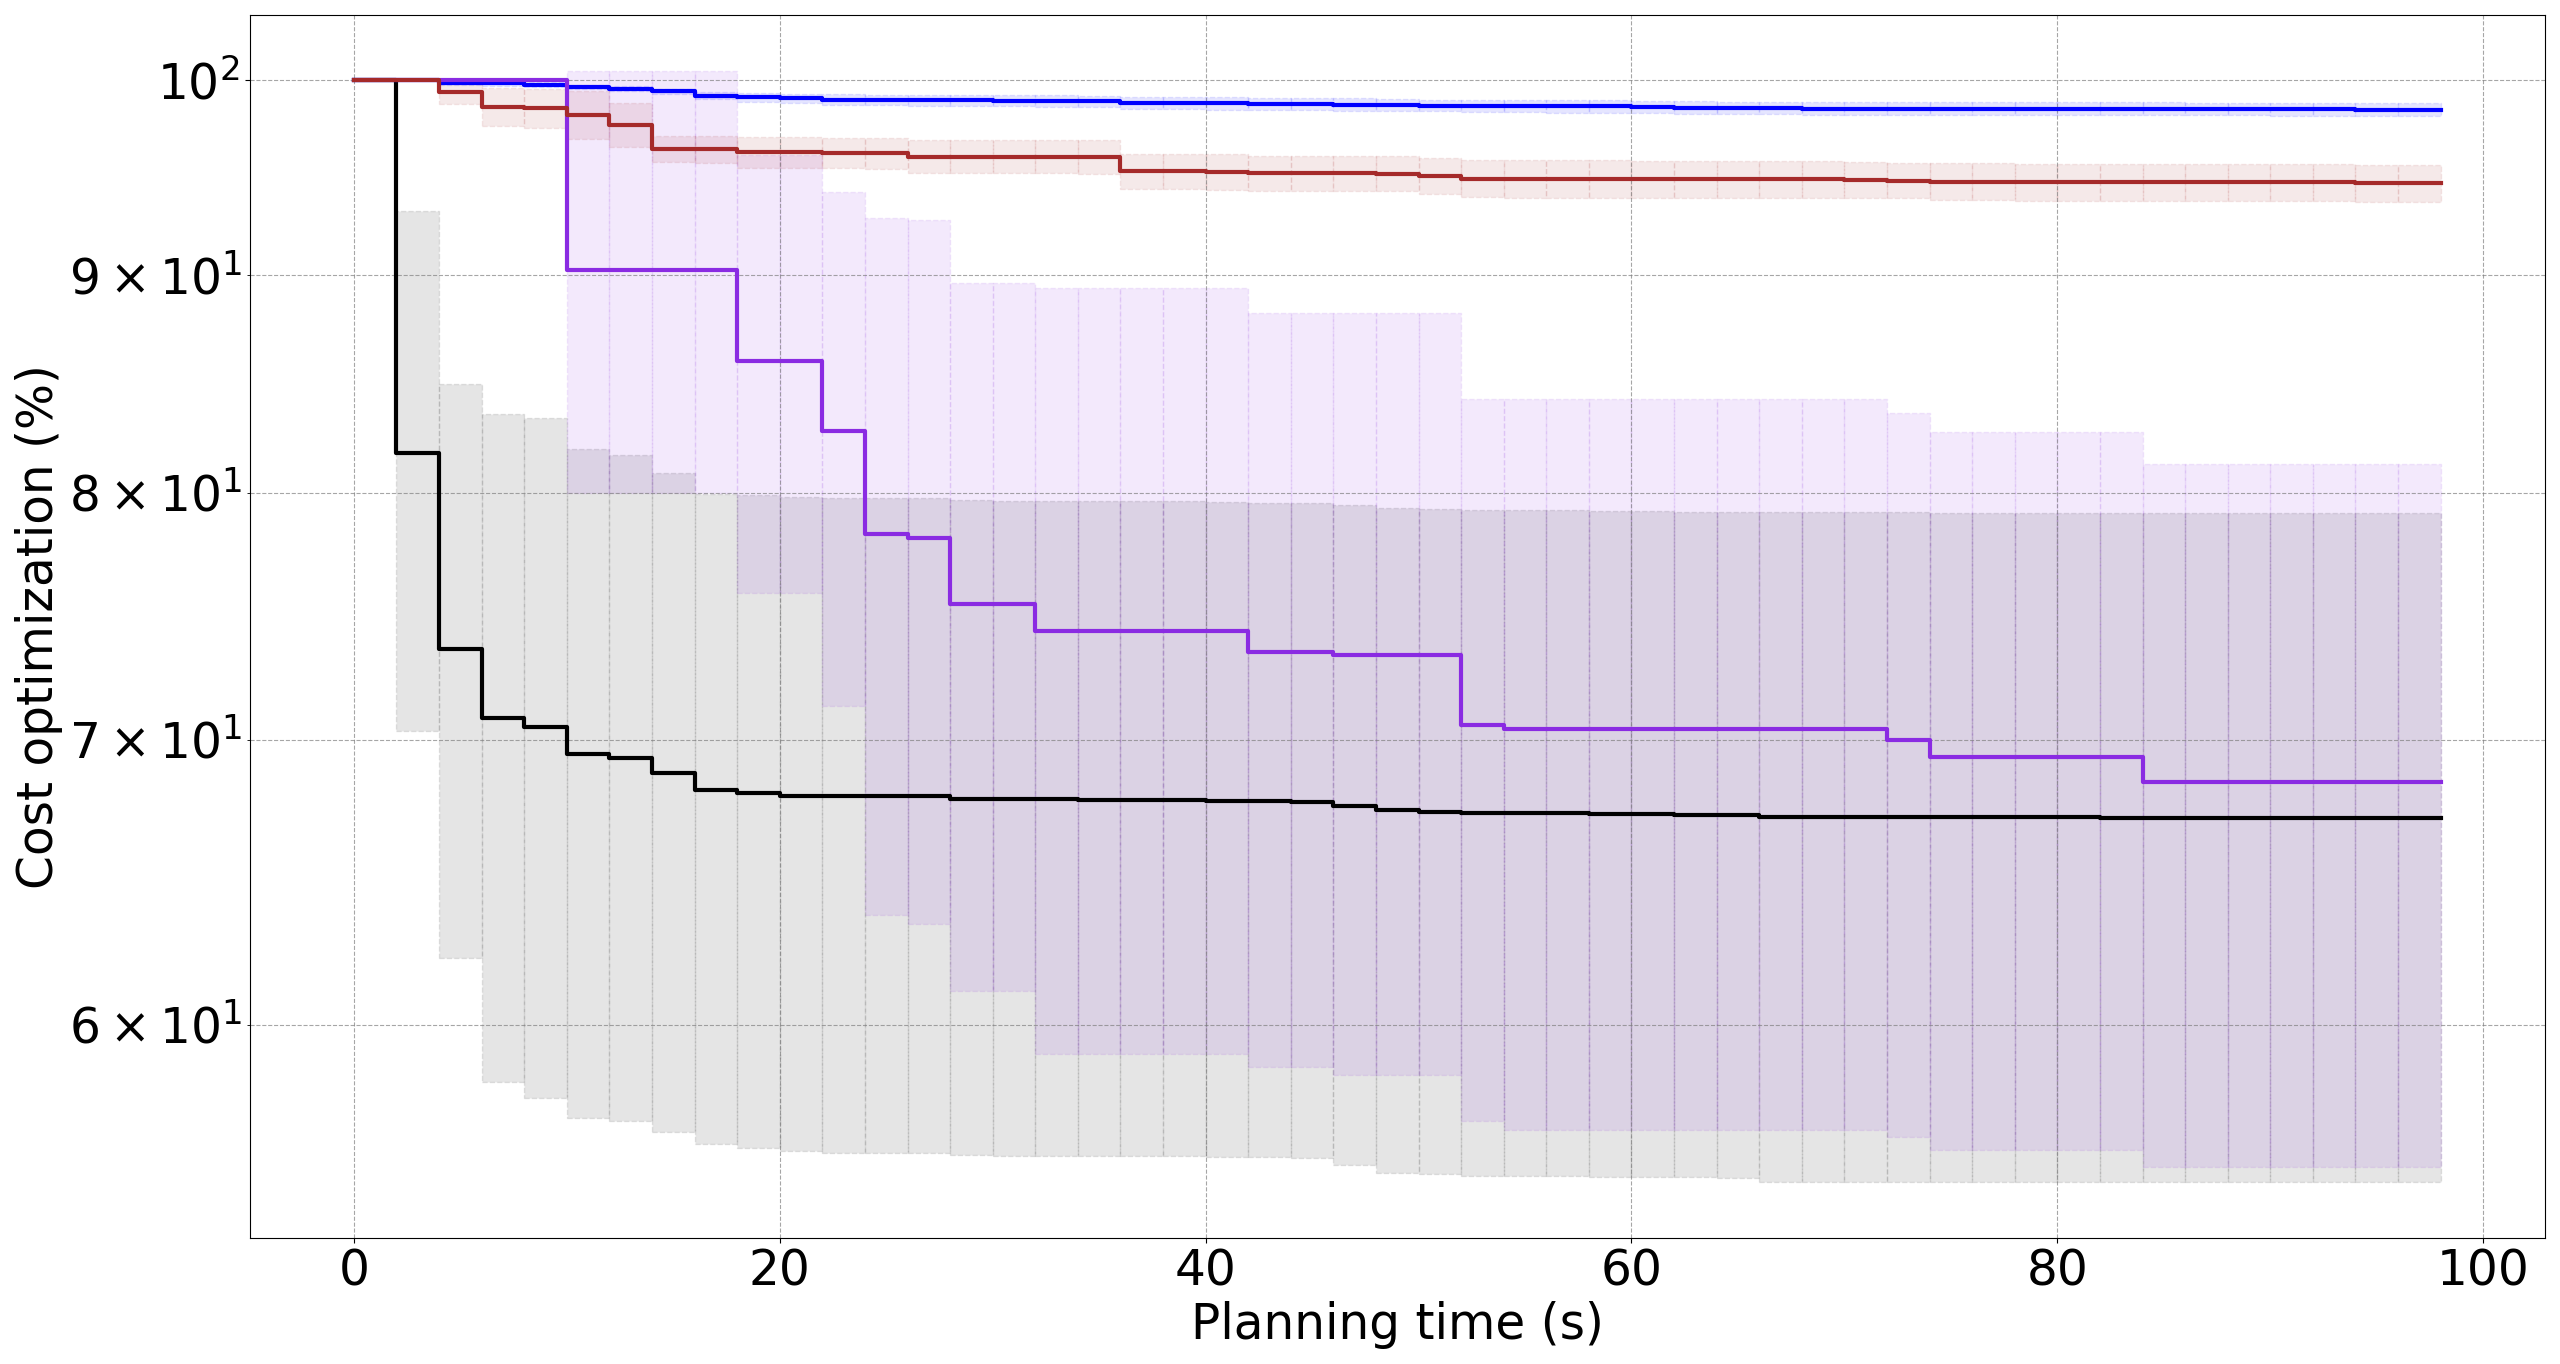
\includegraphics[width=0.9\linewidth]{figures/accuracy/all_methods_window.png} \\
    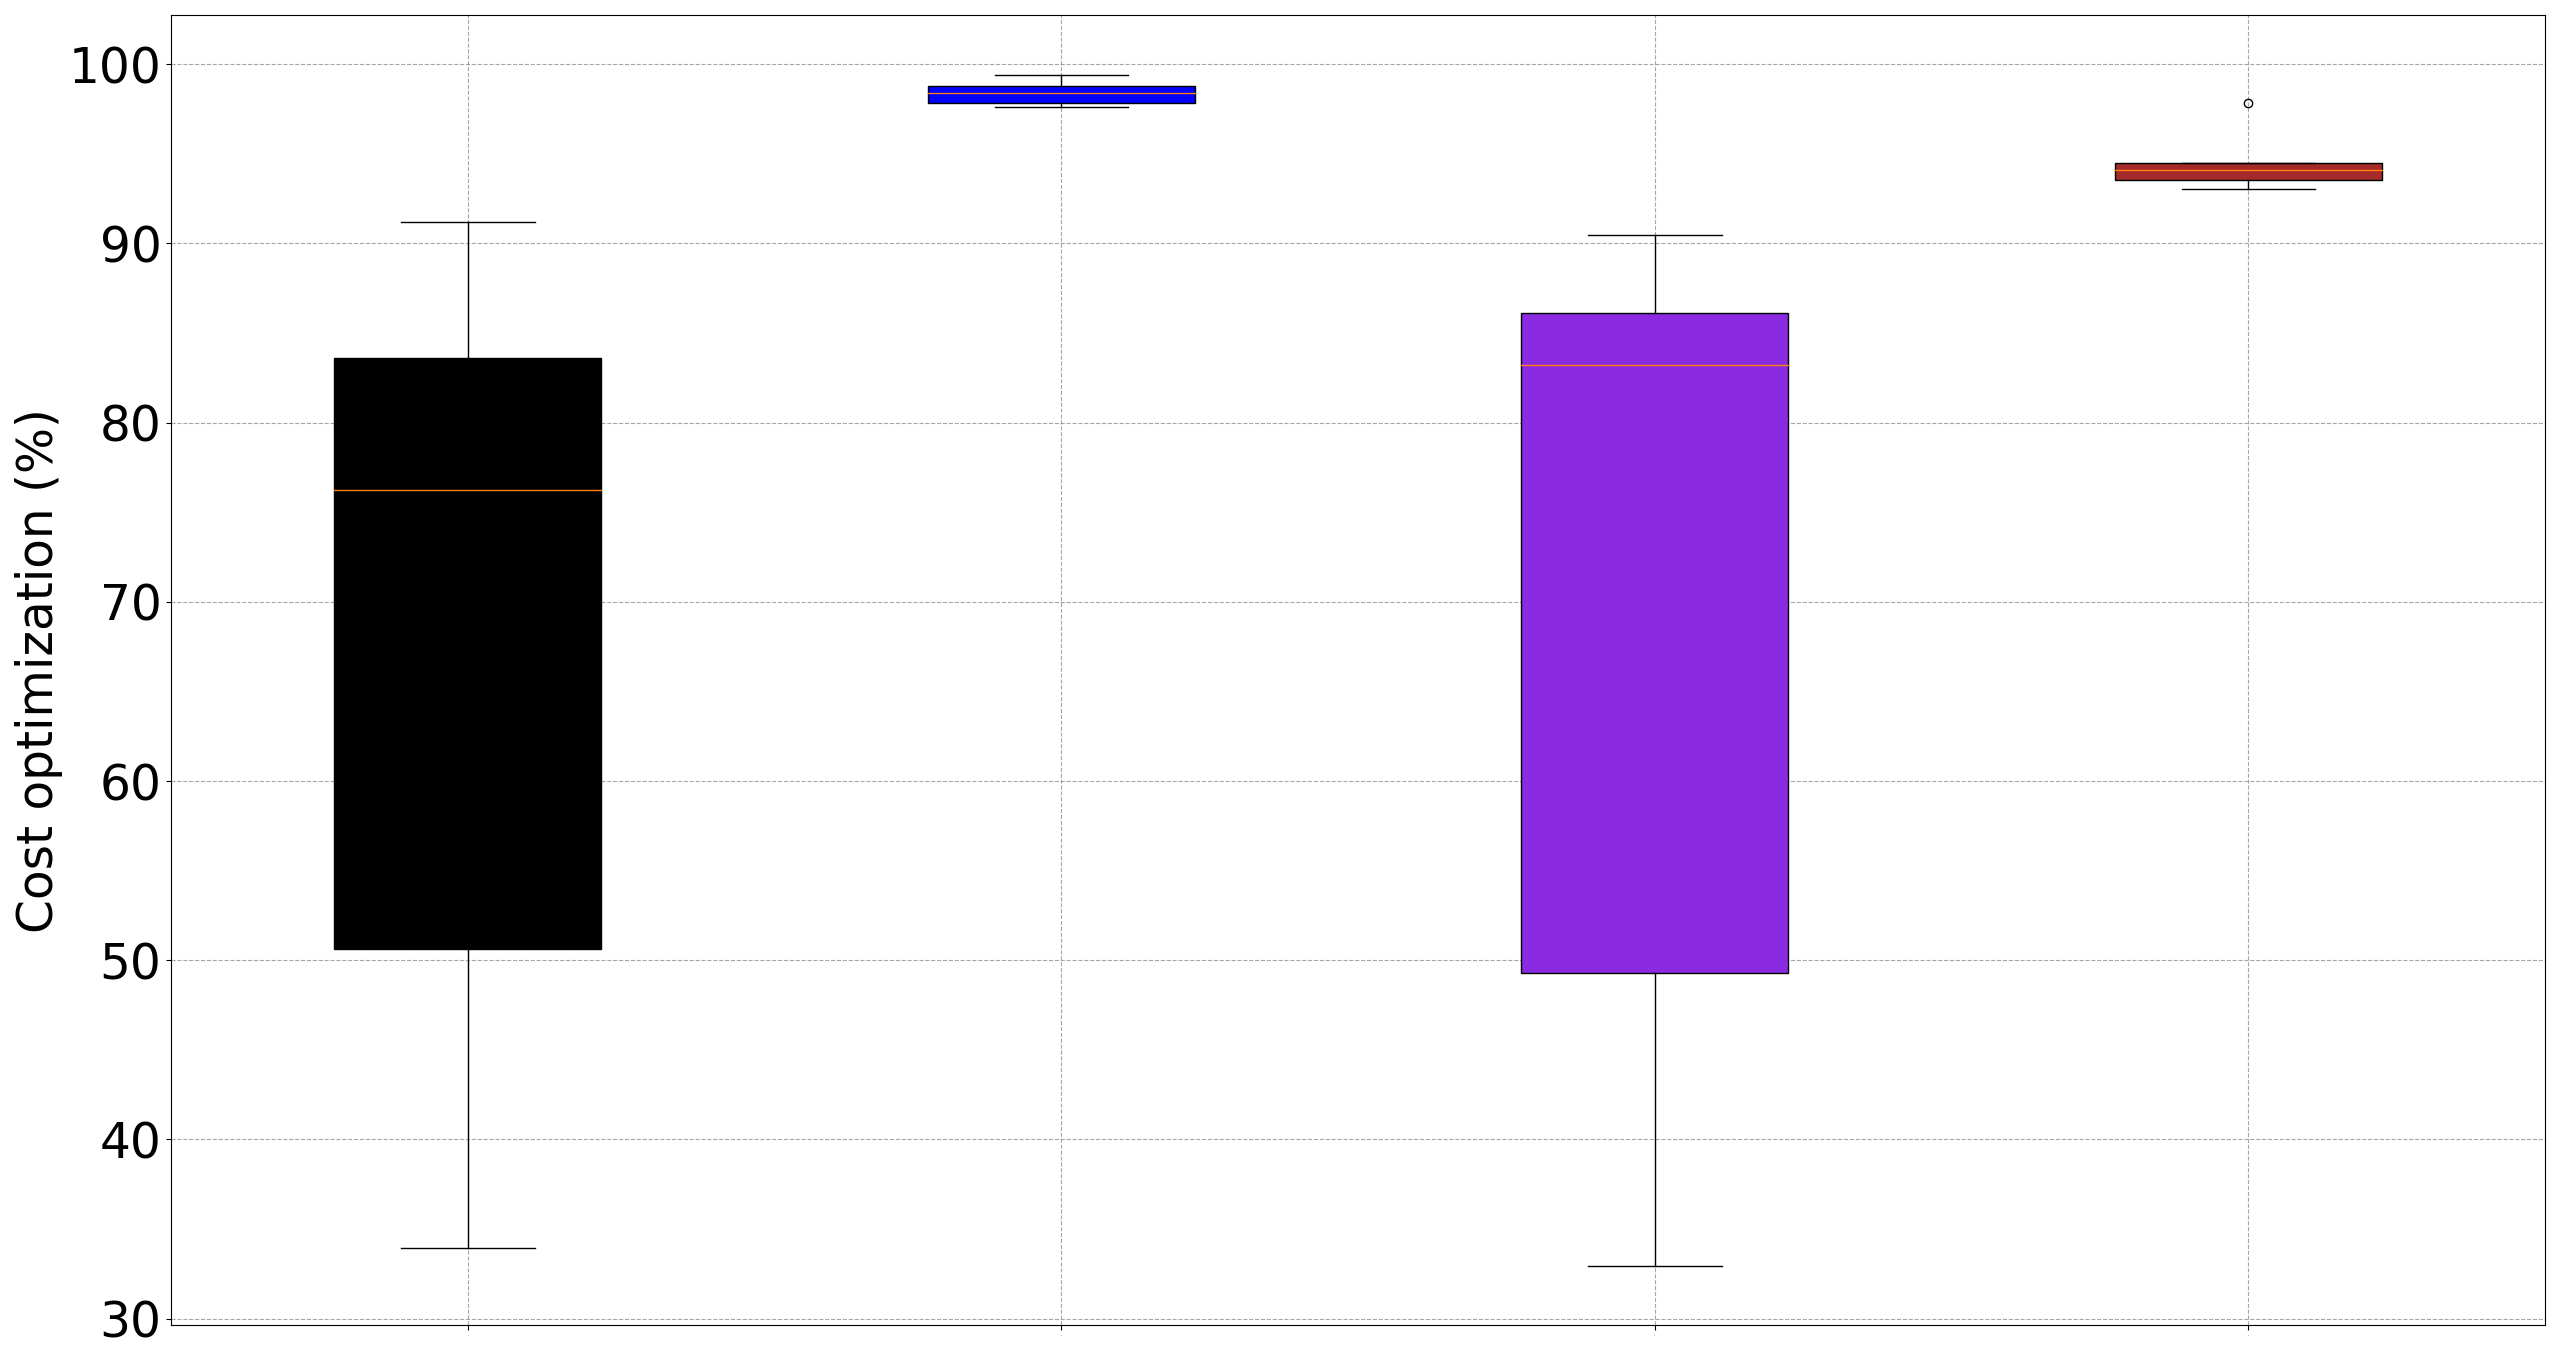
\includegraphics[width=0.9\linewidth]{figures/accuracy/bplot_all_methods_window.png}
    \caption{Cost optimization results for the four methods outlined in Section~\ref{sec:AOptim}, averaged over 10 plans in the window environment. 
    The standard deviation is represented as an envelope around the mean curves.
    The \myglsentry{sastomp} is shown in red, \myglsentry{SAshortcut} in black, \myglsentry{saextendedshct} in purple, and \myglsentry{cobyla} in blue.}%
    \label{fig:acc_window}%
\end{figure}

\paragraph{Corridor environment}

A second environment is also considered, as depicted in Figure~\ref{fig:corridor}, to further analysed the \myglsentry{saextendedshct} sensitivity to its hyperparameters.
The results are illustrated by Figure~\ref{fig:acc_corridor}, where \myglsentry{cobyla} and \myglsentry{sastomp} present the same behavior as previously observed.

The \myglsentry{SAshortcut} achieves the best optimization together with the best convergence rate.
The \myglsentry{saextendedshct} is tested with a Gaussian sampling using two different standard deviation $\delta \in \{0.1, \, 0.01\}$.
The results show that although $\delta = 0.1$ is the best setup to achieve convergence in the obstacle-free environment, it is not the best choice in this case.
This confirms the sensitivity of the algorithm to its hyperparameters.

\begin{figure} [htp]
    \centering
    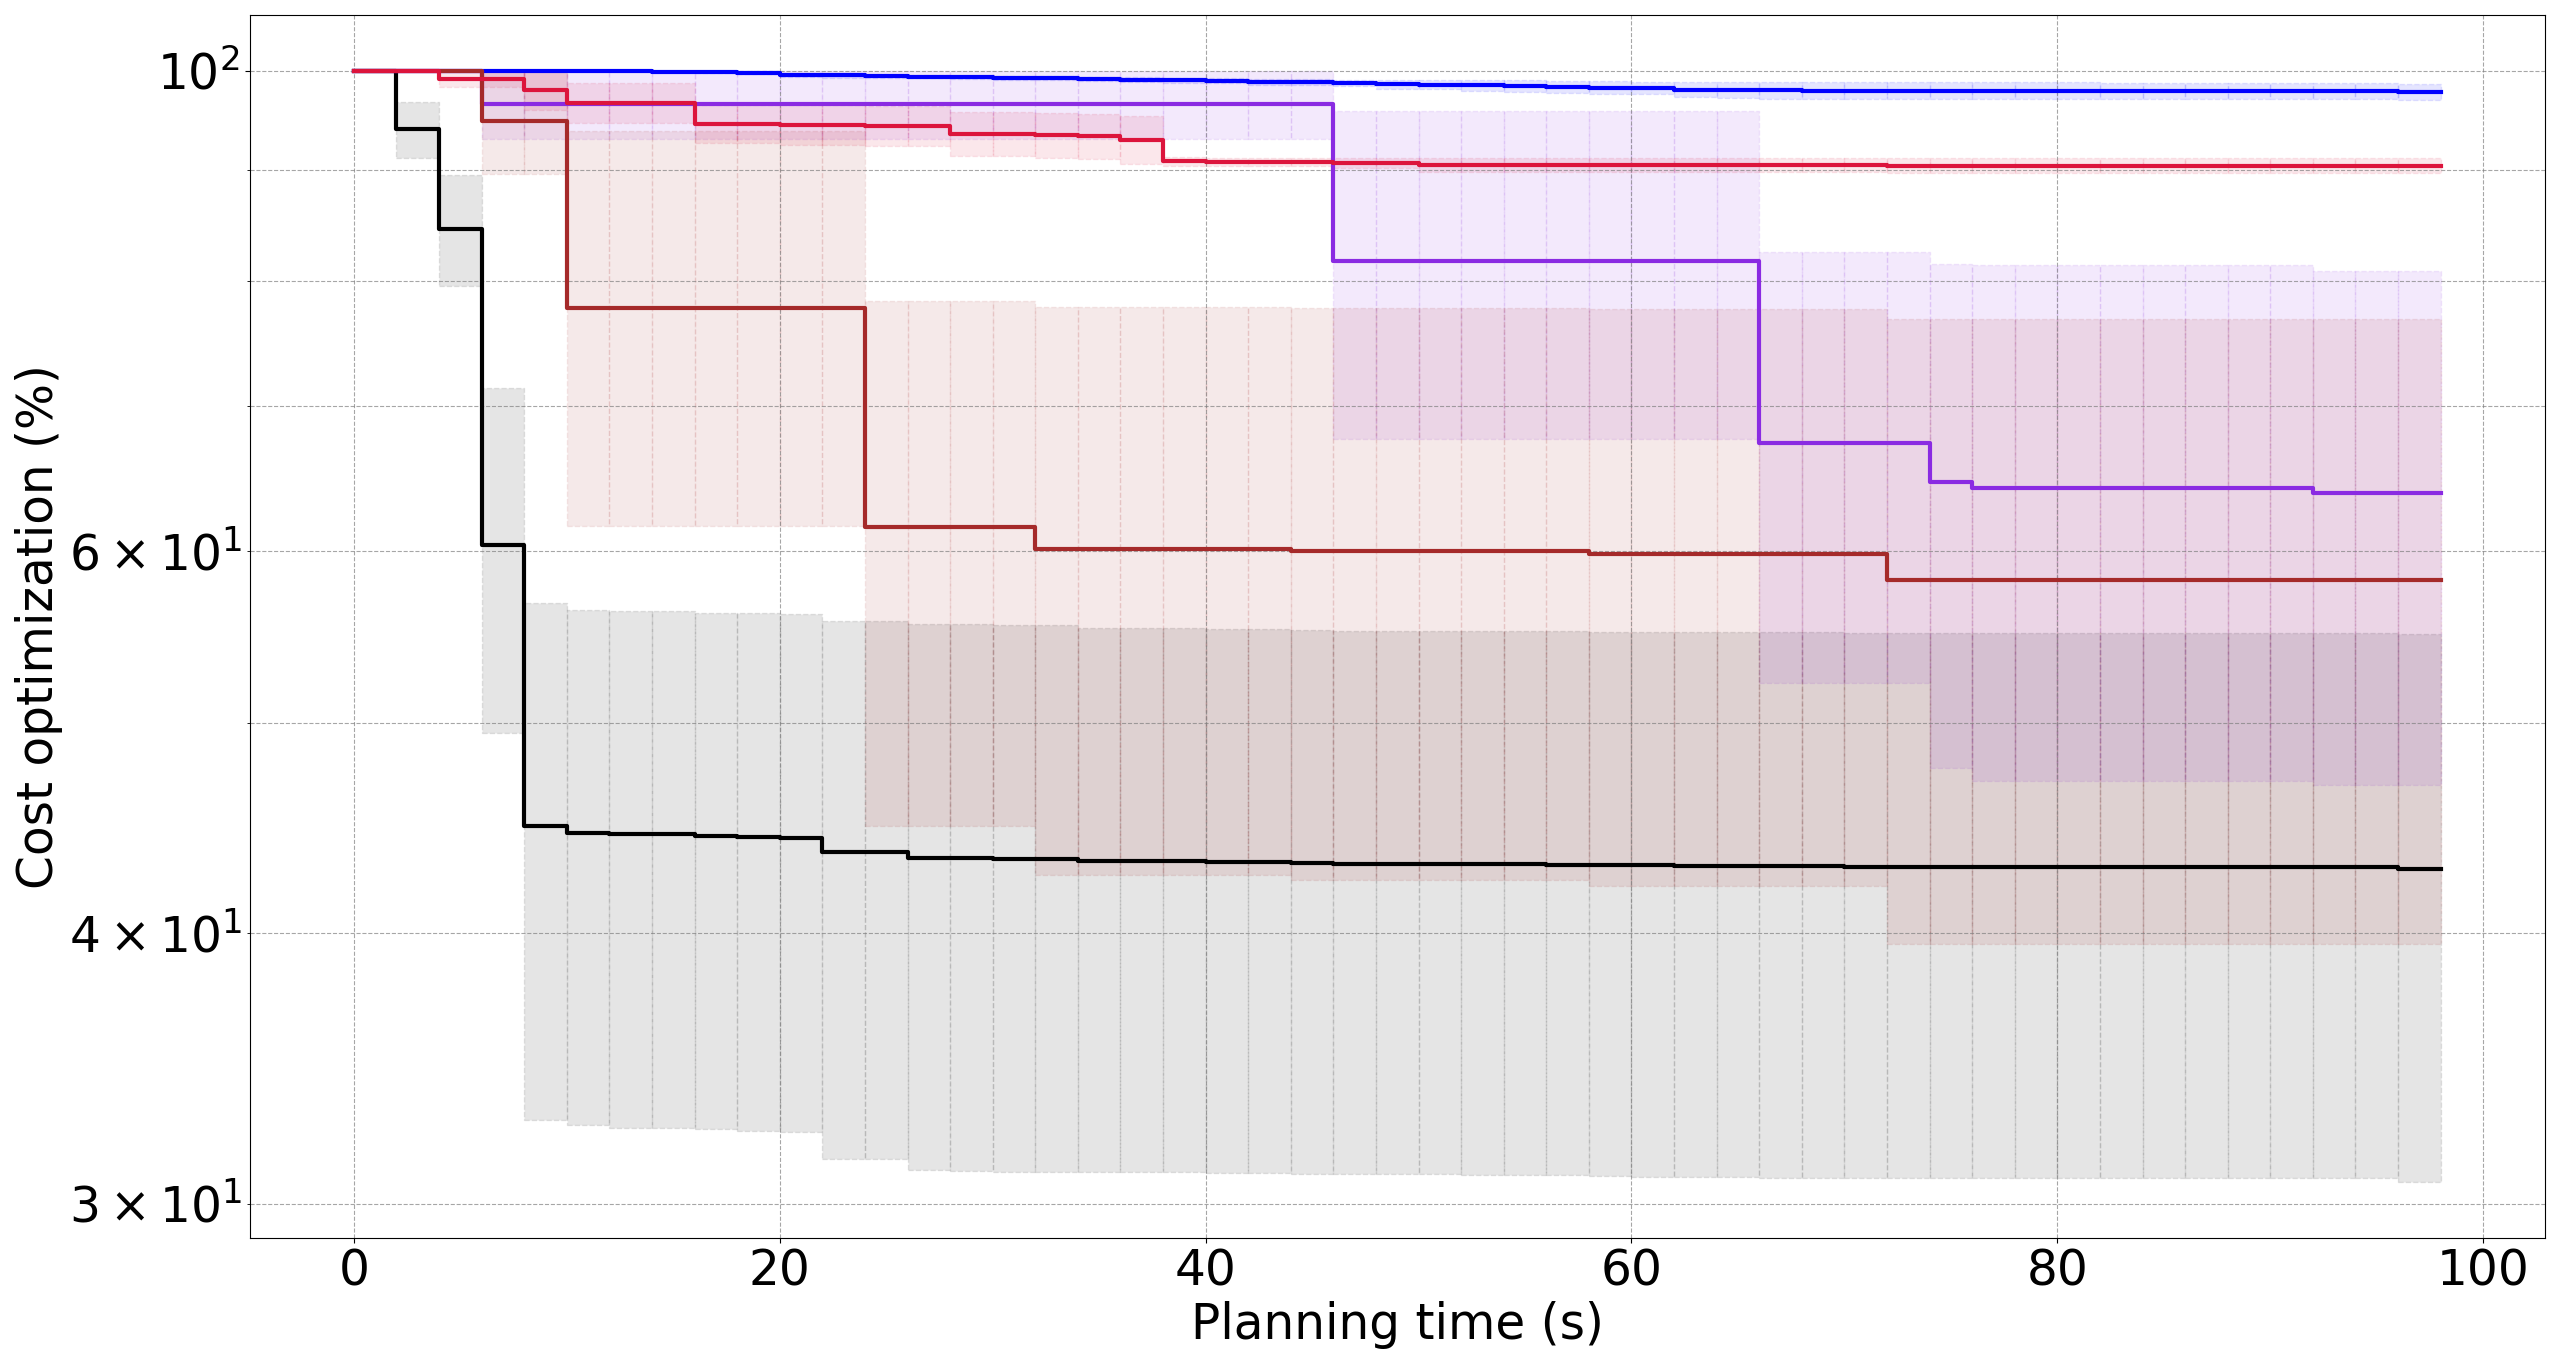
\includegraphics[width=0.9\linewidth]{figures/accuracy/all_methods_corridor.png} \\
    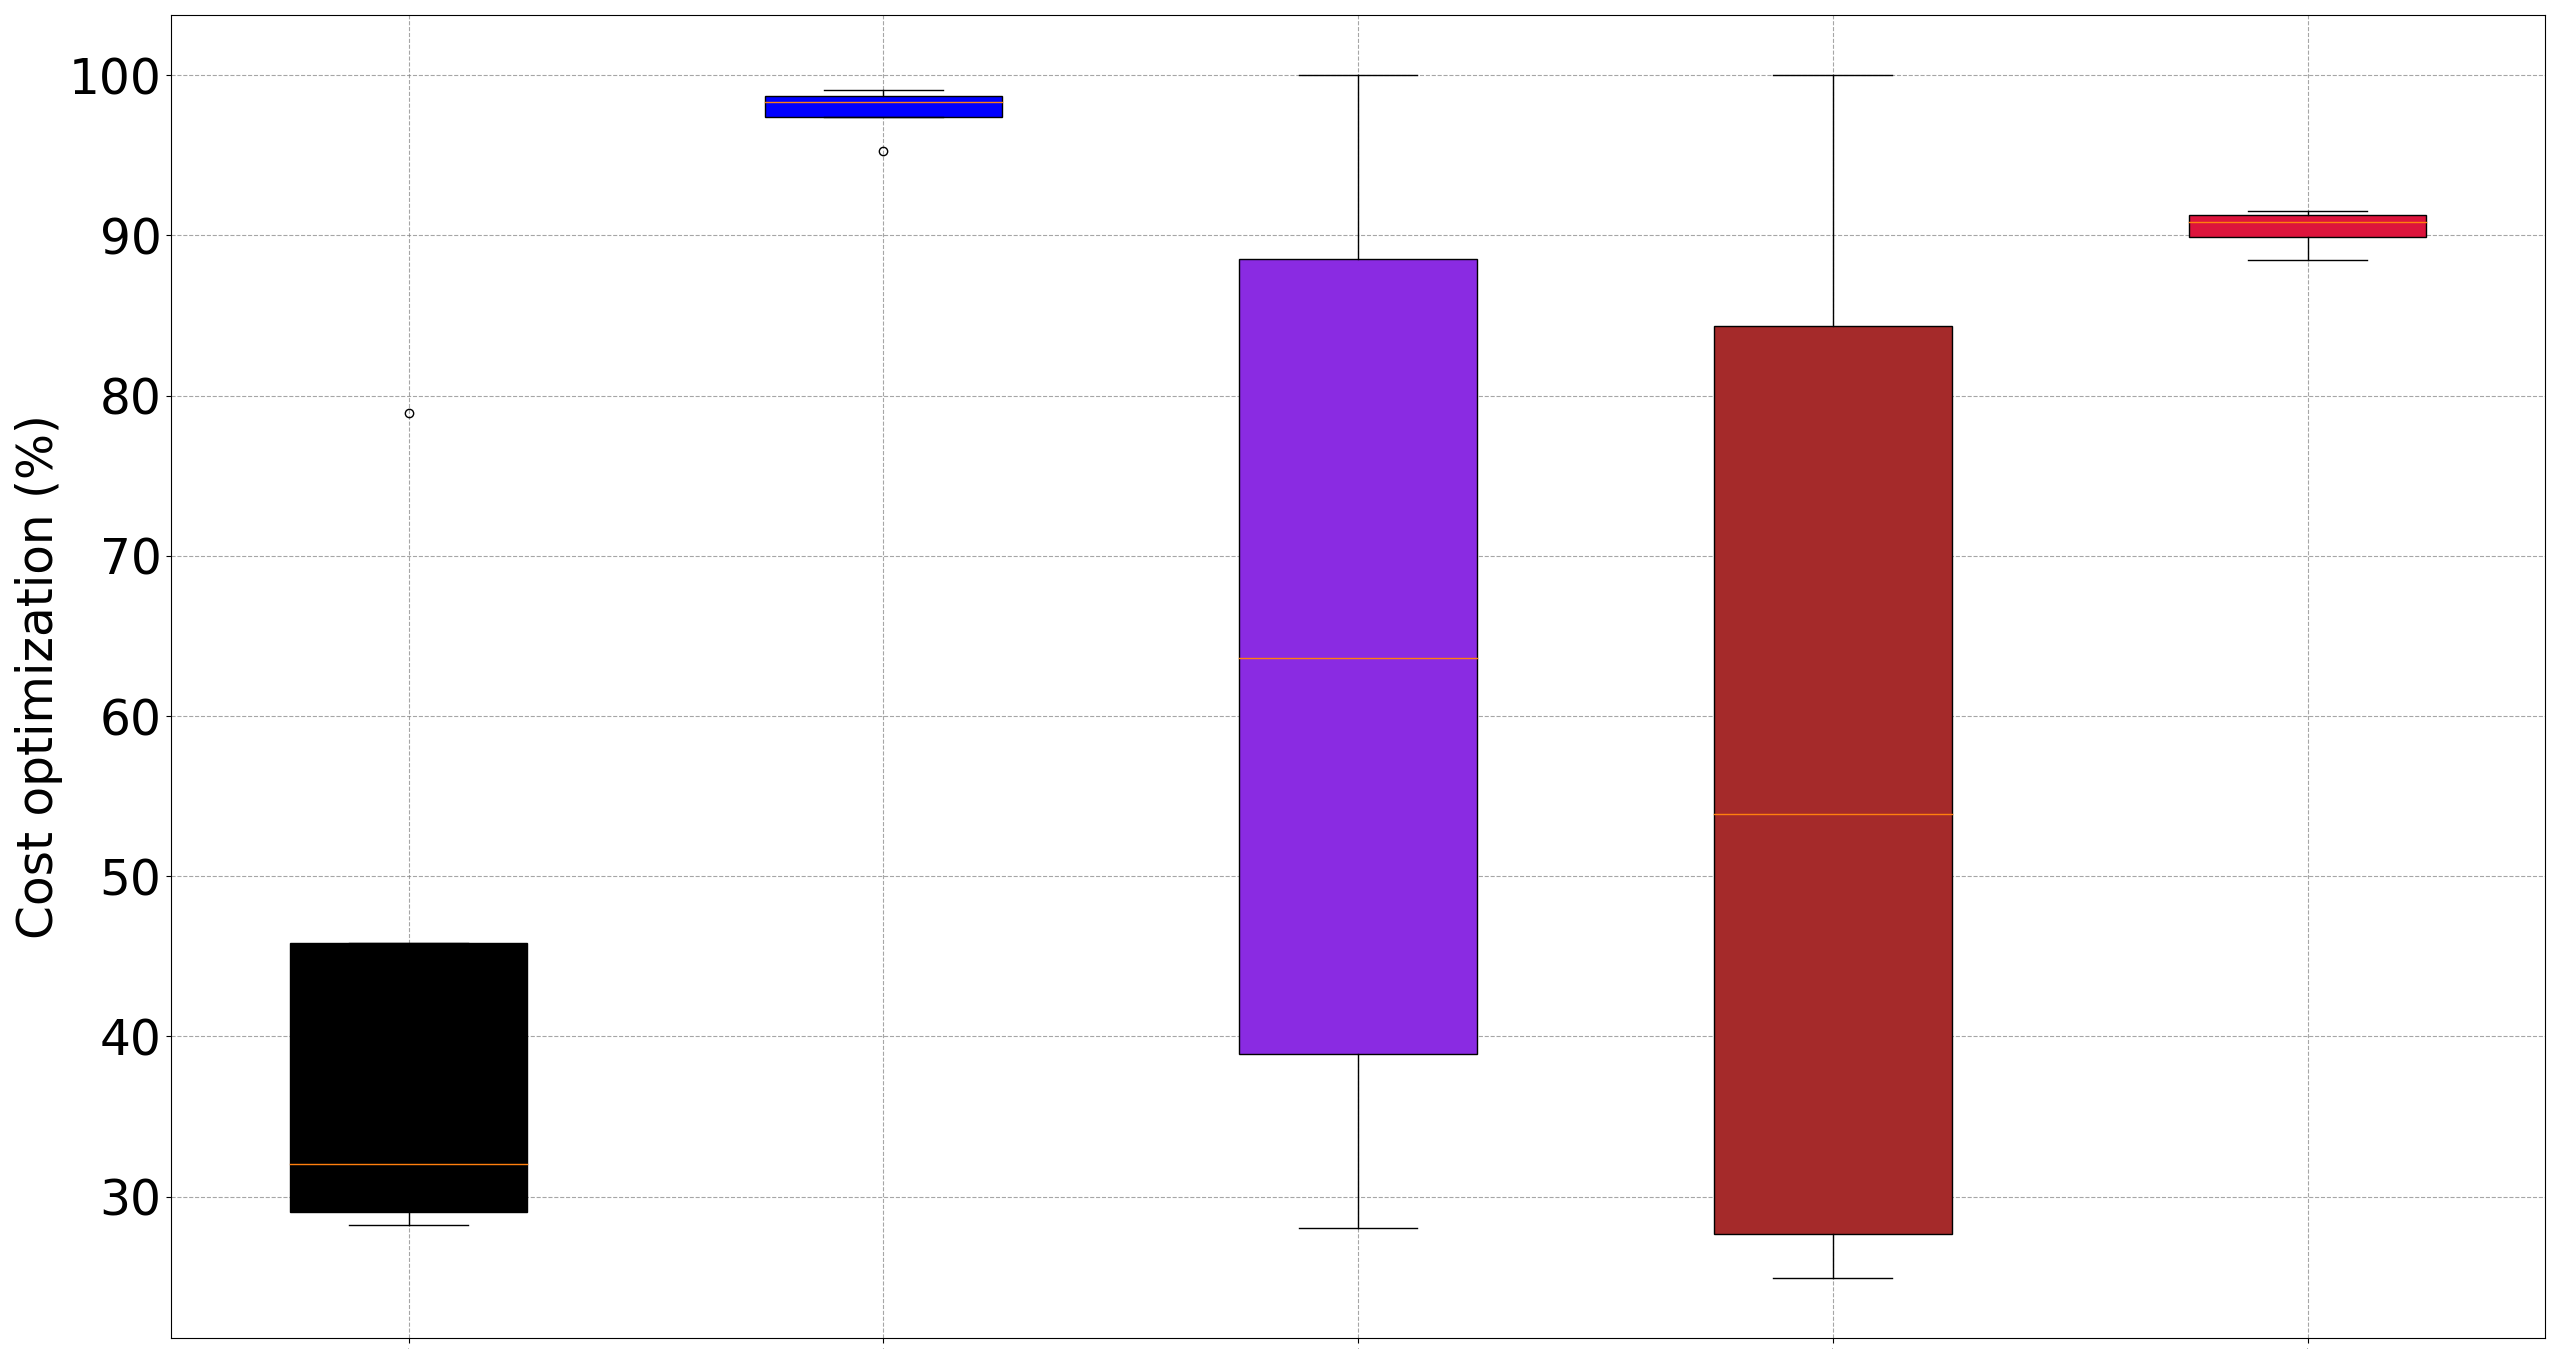
\includegraphics[width=0.9\linewidth]{figures/accuracy/bplot_all_methods_corridor.png}
    \caption{Cost optimization results for the four methods outlined in Section~\ref{sec:AOptim}, averaged over 10 plans in the corridor environment. 
    The standard deviation is represented as an envelope around the mean curves.
    The \myglsentry{sastomp} is shown in red, \myglsentry{SAshortcut} in black, and \myglsentry{cobyla} in blue.
    Two \myglsentry{saextendedshct} setup are considered: both use a Gaussian sampling with $K = 1$, but the purple curve uses a standard deviation of $\delta = 0.1$, while the brown one uses $\delta = 0.01$}%
    \label{fig:acc_corridor}%
\end{figure}

\paragraph{Controller gains optimization}

While the robust local optimizers compared above consider only the trajectory states as optimization variables, the work in~\cite{AliIROS} demonstrates that optimizing both the states and controller gains achieves the best accuracy performance.
Therefore, \myglsentry{SAshortcut} has been implemented such that, at each iteration, a shortcut is attempted between two states of the input trajectory, randomly sampled along with controller gain values, which are chosen within 50\% to 150\% of their nominal values (see Section~\ref{sec:quad_setup}).
Figure~\ref{fig: Acc opti} motivates why we optimized both the trajectory and the controller gains at the same time in the A-Optim function in order to minimize uncertainty for a given point, as mentioned in Section~\ref{sec:RASAMP}. 
In fact, these results corroborate the findings of \cite{AliIROS}, but this time by employing a sampling-based motion planner that considers obstacles in the environment.

\begin{figure} [htp]
    \centering
    {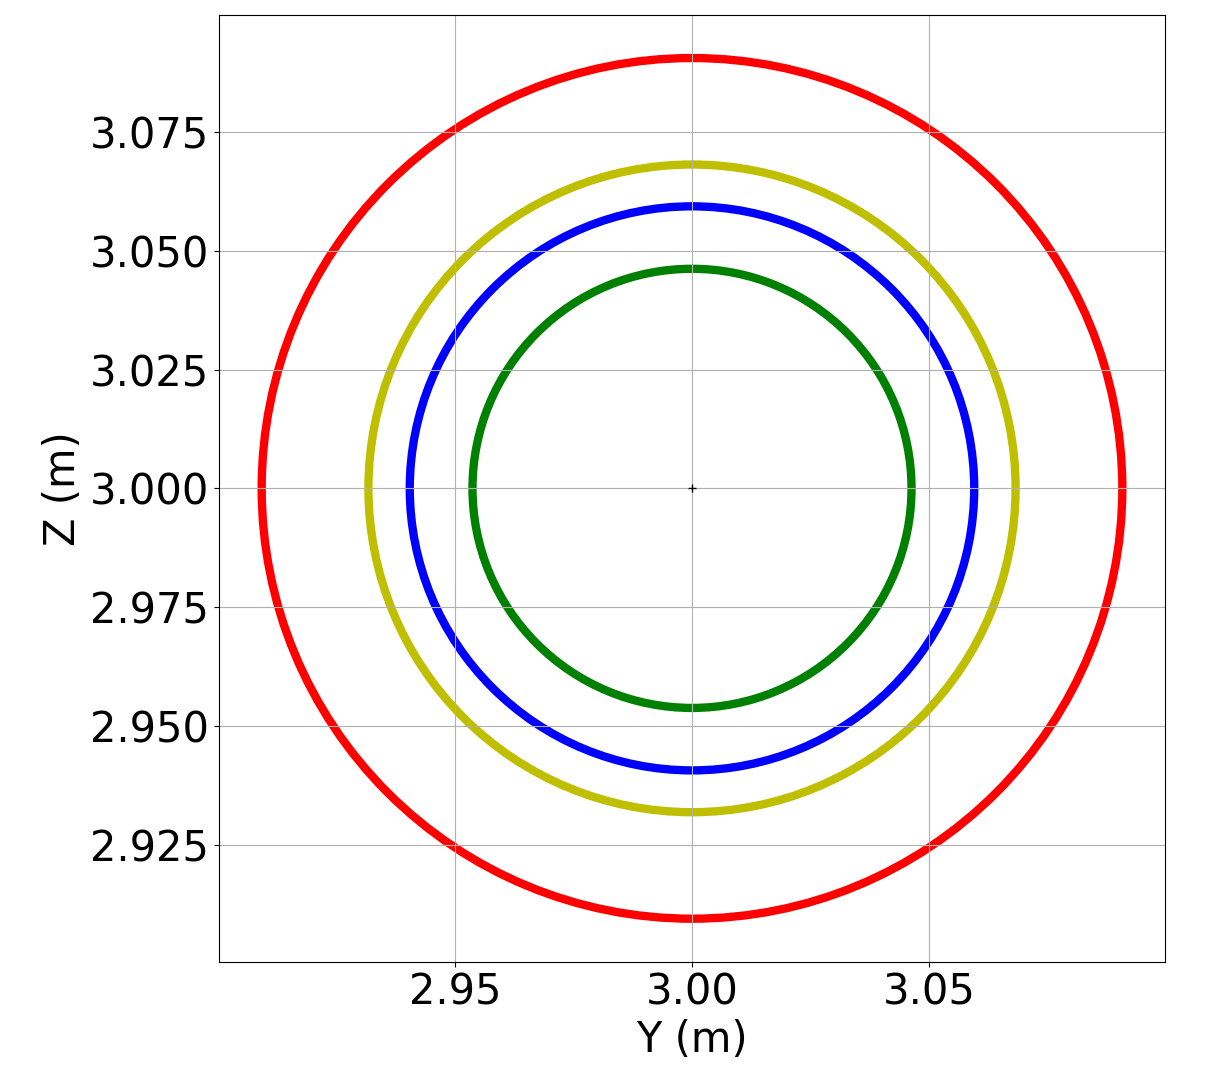
\includegraphics[width=0.5\linewidth]{figures/robust_accurate/accuracy_opti.png} }%
    \caption{Example of uncertainty ellipsoid without optimization (red), with local trajectory optimization (yellow), with gains optimization (blue), and with local trajectory and gains optimization at the same time (green).}%
    \label{fig: Acc opti}%
\end{figure}

\paragraph{Conclusion}

The \myglsentry{cobyla} algorithm remains highly localized to the vicinity of the reference trajectory, while \myglsentry{sastomp} exhibits a very slow convergence rate.
Although \myglsentry{saextendedshct} was designed to enable better exploration of the cost space compared to \myglsentry{SAshortcut}, while maintaining an efficient convergence rate, it proves challenging to tune effectively.
Therefore, in the following experimental section, the A-Optim method of the meta algorithm of Section~\ref{sec:RASAMP} is performed using \myglsentry{SAshortcut} considering both the trajectory states and controller gains as optimization variables.

Recall that, because the GRU is trained for specific controller gains, and the trajectories encountered during the \myglsentry{SAshortcut} process deviate significantly from those used during training, \myglsentry{SAshortcut} does not benefit from the neural network.

\section{Experimental validation} \label{sec:Experimental}

This section provides an experimental validation of both the deep learning-based robust motion planning variants, and the accuracy optimization stage in two challenging scenarios depicted in Figure~\ref{fig: Missed and succes}.

\begin{figure} [htp]
    \centering
    \subfloat[\centering Robust motion planning]{{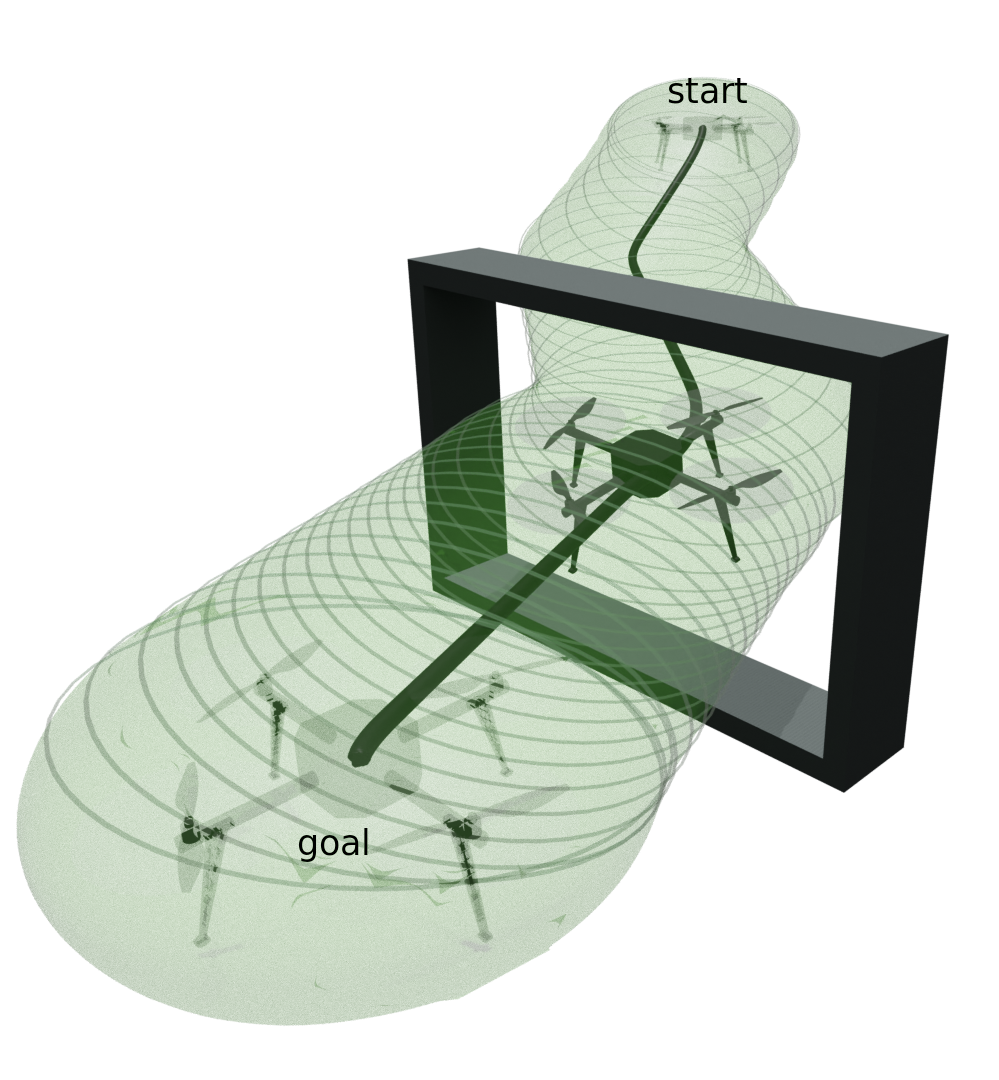
\includegraphics[width=0.4\linewidth]{figures/robust_accurate/topFig_tube.png} }\label{fig: fig1robust}}%
    \subfloat[\centering Accuracy optimization]{{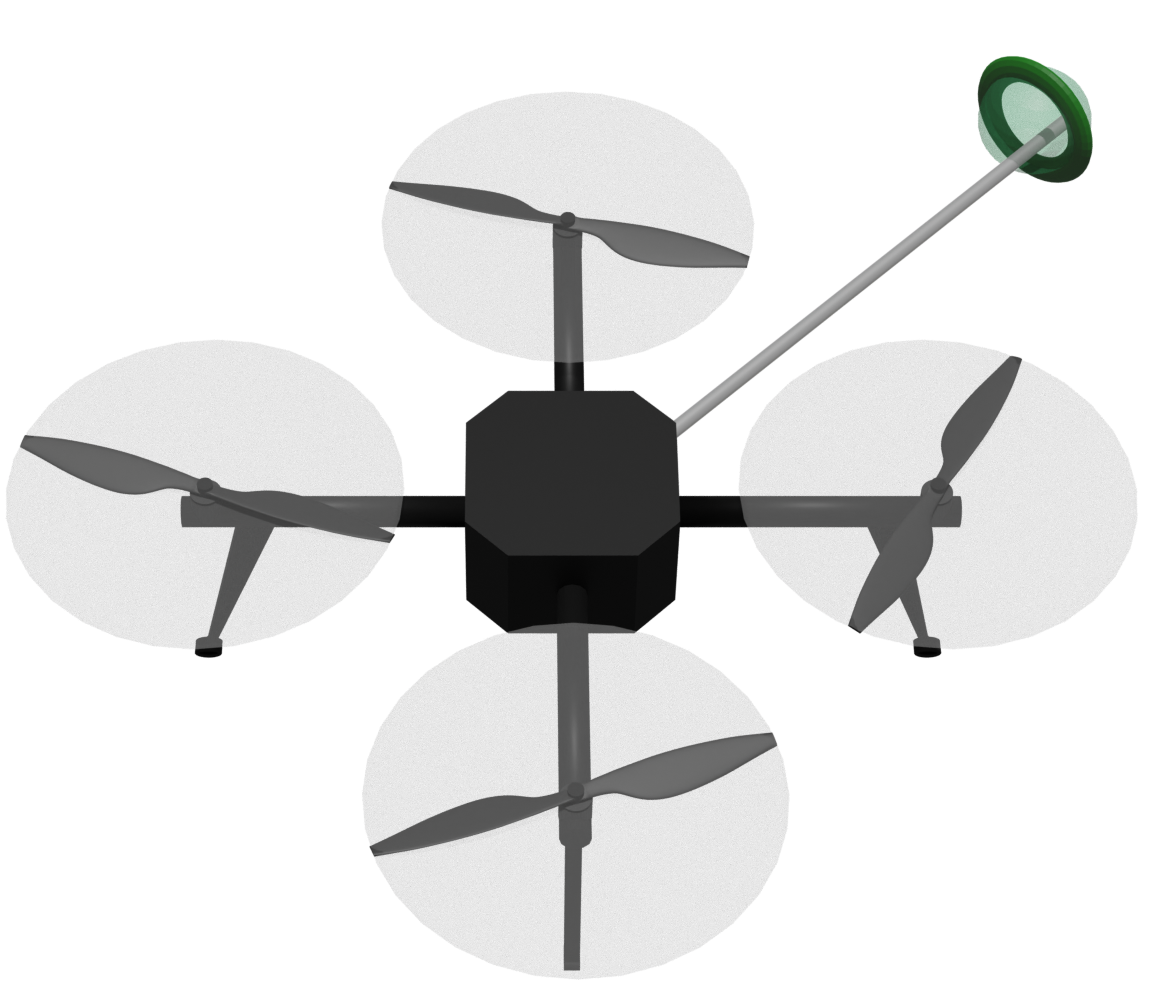
\includegraphics[width=0.4\linewidth]{figures/robust_accurate/ring_success.png} } \label{fig: fig1acc}}%
    \caption{
    Two scenarios considered for the experimental validation of the proposed method:
    (a) Robust navigation of a drone through a narrow window. (b) Precision in-flight `ring catching' task, where the uncertainty on the position of the perch end-effector is minimized to successfully accomplish the task.
    A video of the experiments is available at: \href{https://laas.hal.science/hal-04642257}{https://laas.hal.science/hal-04642257}}%
    \label{fig: Missed and succes}%
\end{figure}

\begin{figure} [htp]
    \centering
    
    \subfloat[\centering ]{{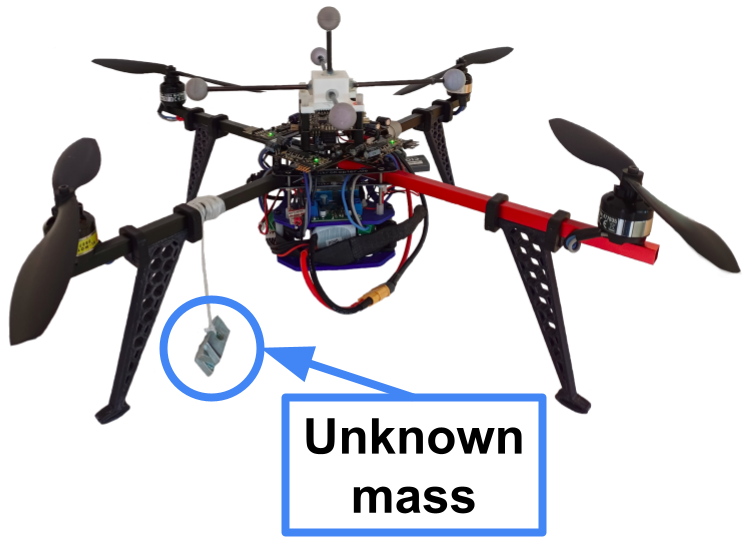
\includegraphics[width=0.42\linewidth]{figures/robust_accurate/drone_window.png} }\label{fig: drone_mass}}%
    \subfloat[\centering ]{{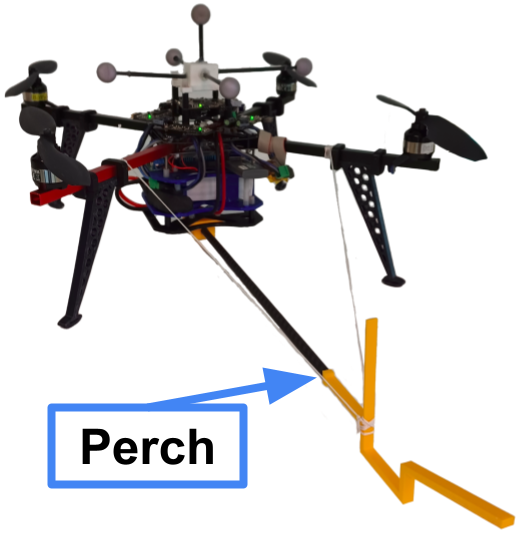
\includegraphics[width=0.3\linewidth]{figures/robust_accurate/drone_perch.png}} \label{fig: drone_perch}} \\%
    \subfloat[\centering ]{{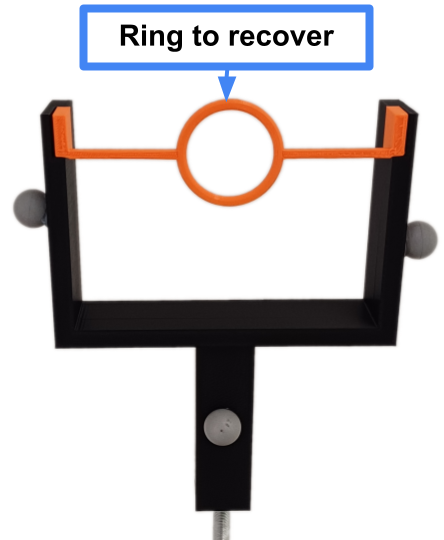
\includegraphics[width=0.3\linewidth]{figures/robust_accurate/ring.png}} \label{fig: ring}}
    \caption{Quadrotor setups for the two scenarios considered for the experimental validation. (a) a drone equipped with a random mass to perform a robust navigation through a window (b) a drone equipped with a perch to catch (c) the rings.}%
    \label{fig: exp setup}%
\end{figure}

\subsection{Robust planning} \label{sec:RobustPlanExp}

The window scenario, depicted in Figure~\ref{fig: fig1robust} and evaluated in simulation in Section~\ref{sec:RobustPlanSimu}, is experimentally validated on a real quadrotor.
In this scenario, uncertainties are added to the system by randomly attaching a mass of up to 80g (not known by the controller) to the drone as depicted in Figure~\ref{fig: drone_mass}.

In this experiment, a non-robust trajectory planned by RRT* and a robust one planned by DeepSARRT* were executed ten times, using the same masses and attachment points between the two algorithms.
All trajectories were planned offline on a remote computer. 
To make the robot execute them, the geometric controller~\cite{cLee} ran online on the quadrotor onboard computer, tracking the trajectories provided as input thanks to the Genom3 software~\cite{cGenom3}. 
The robot state was measured using a motion capture system with millimeter accuracy, ensuring that the only source of uncertainty was the attached unknown mass.
Figure~\ref{fig: exp window} illustrates the experimental execution of a non-robust RRT* trajectory and a robust DeepSARRT* trajectory. 
The figure shows the recorded executions within a virtual environment to detect virtual collisions, thus mitigating the risk of real crashes and damages to the robot.
The experimental results confirm the simulation observations, providing an overall success rate of 100\% in the case of the robust trajectory computed with DeepSARRT*, against 40\% for the classic RRT*.

\begin{figure} [htp]
    \centering
    \subfloat[\centering RRT*]{{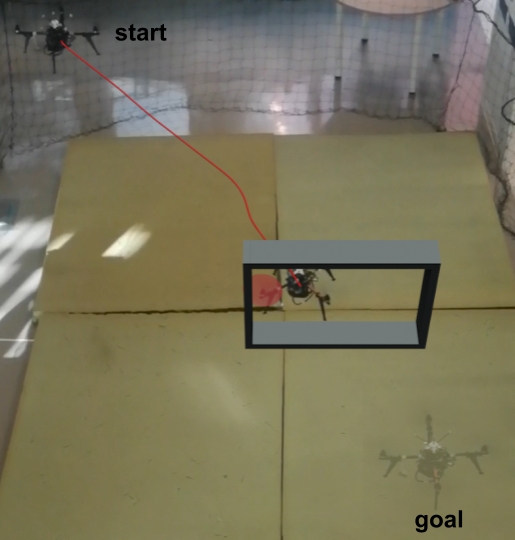
\includegraphics[width=0.4\linewidth]{figures/robust_accurate/exp_RRTstar.png} }}%
    \subfloat[\centering DeepSARRT*]{{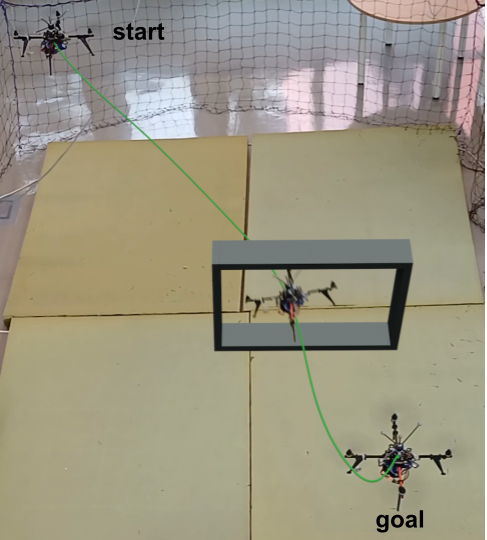
\includegraphics[width=0.378\linewidth]{figures/robust_accurate/exp_SARRTstar.png} }}%
    \caption{Experimental execution by a quadrotor with uncertainty of trajectories planned by RRT* (a) and DeepSARRT* (b). 
    Both trajectories are executed with the same uncertainty and a virtual collision is found in the RRT* case while the DeepSARRT* execution is robust.}%
    \label{fig: exp window}%
\end{figure}

\subsection{Accuracy optimization} \label{sec:AccOptExp}

\begin{figure} [htp]
    \begin{subfigure}{0.63\linewidth}
      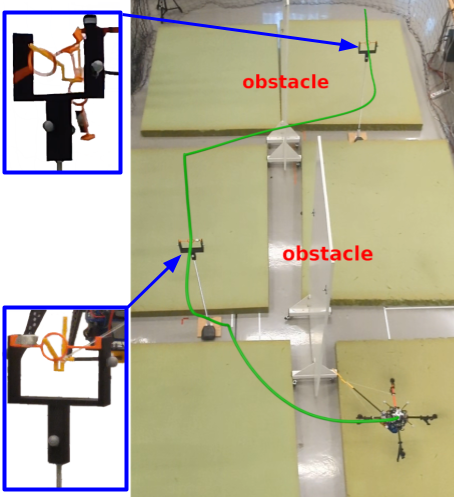
\includegraphics[width=\linewidth]{figures/robust_accurate/ring_opti_v1.png}
    \end{subfigure}\hfill
    \begin{subfigure}{0.37\linewidth}
        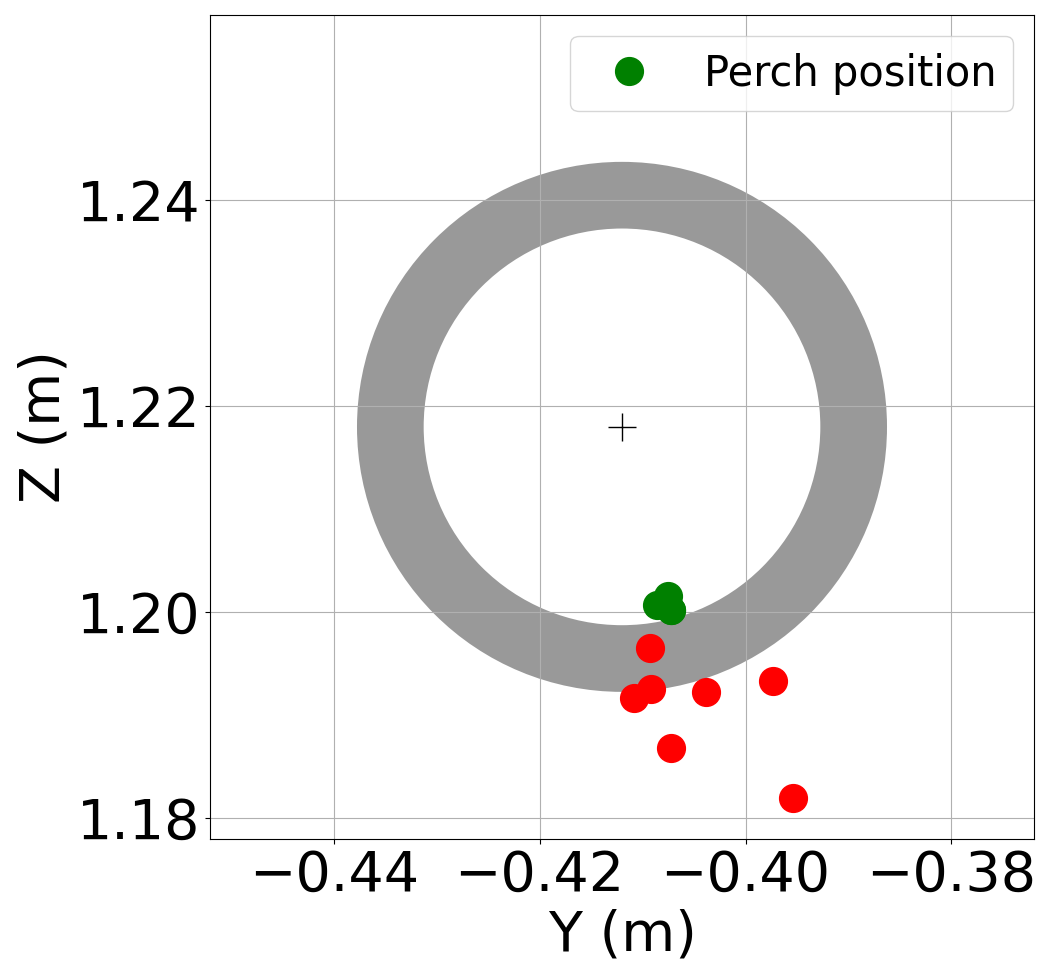
\includegraphics[width=\linewidth]{figures/robust_accurate/Exp_ring_no_opti_full_zoom.png}
        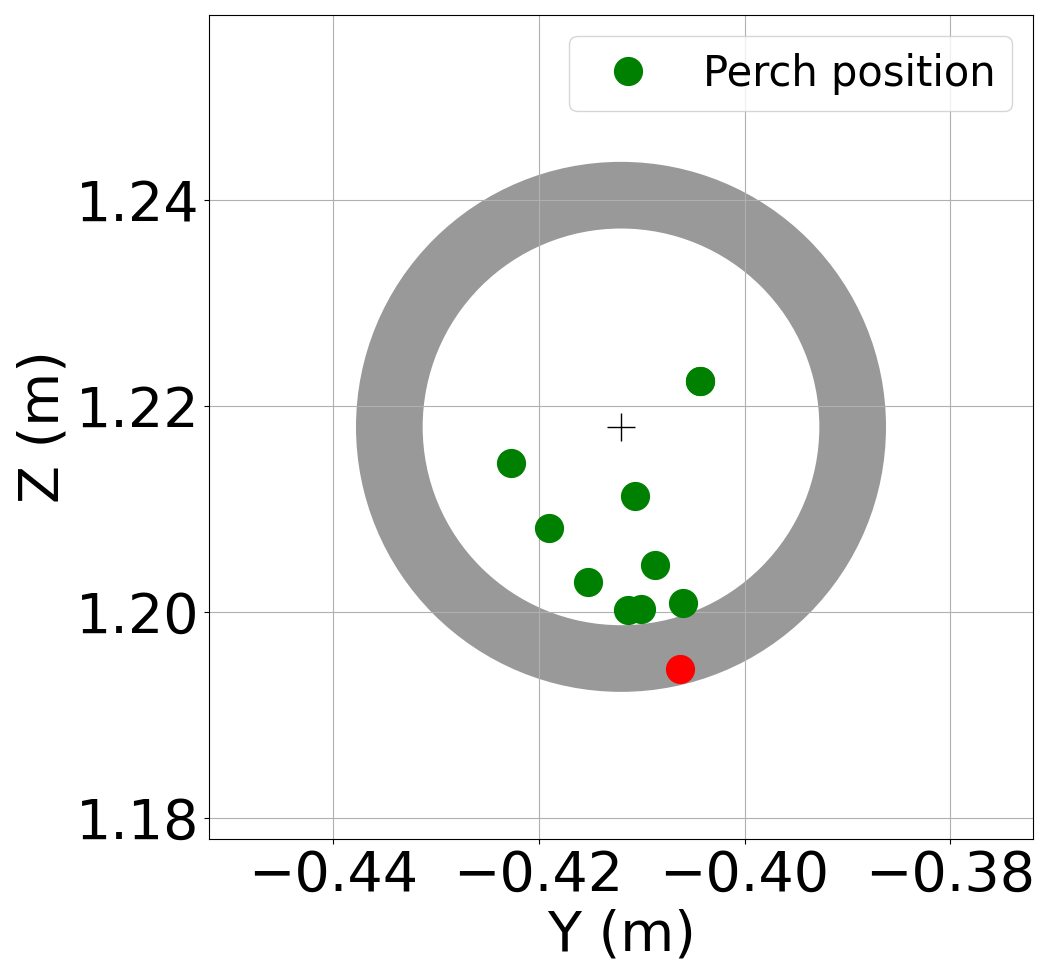
\includegraphics[width=\linewidth]{figures/robust_accurate/Exp_ring_opti_full_zoom.png}
    \end{subfigure}\hfill
    
\caption{Experimental validation of the ``ring catching'' scenario with a perch-equipped drone (left) with the position of the perch end-effector at the second ring location over 10 trajectories non accuracy optimized (top right) and accuracy optimized (bottom right).}
\label{fig: exp ring}
\end{figure}

A second experimental scenario is presented in order to evaluate the complete framework presented in Section~\ref{sec:RASAMP}.
This scenario involves a challenging in-flight retrieval of two 2 cm radius rings in a cluttered environment using a drone equipped with a perch (see Figure~\ref{fig: drone_perch}) in a robust (near) time optimal way.
Note that, unlike the first experimental scenario described earlier, the uncertainties in the system parameters in this case arise from the task itself, specifically during the recovery of the rings.

The experimental setup is shown in Figure~\ref{fig: exp ring}, where the quadrotor is equipped with a perch of 50 cm length, aligned at a 45° angle relative to the body frame x and y axes.
The positions and orientations of the rings are recovered before the planning process using a motion capture system, as depicted in Figure~\ref{fig: ring}.
Based on the positions and orientations of the rings, desired quadrotor states (as for the states in $list_{d}$ in Section~\ref{sec:RASAMP}) is computed to ensure that the incidence angle of the perch is perpendicular to the rings during capture, with zero acceleration.

10 trajectories were planned using a vanilla (non-robust) RRT* planner and the DeepSARRT* algorithm, both designed to optimize trajectory time, and then executed by the real quadrotor.
The RRT* does not use the A-Optim method to optimize accuracy while the DeepSARRT* does, in addition to guaranteeing the robustness.
The offline optimization in A-Optim aimed at minimizing the uncertainty at the location of the two rings.

The first ring is weighted between 10 g and 50 g, so when it is caught, it becomes part of the drone and modifies the overall mass/inertia and center of mass of the system in an unmodeled way. 
Note that the rings are recovered on the perch, which is located at the origin of the z-axis in the body frame. 
Consequently, it is assumed that catching the rings does not introduce any uncertainties in the center of mass along the z-axis. 
Therefore, this is why only shifts along the x and y axes are taken into account in the setup (see Section~\ref{sec:quad_setup}).
Note that, to minimize the impact of catching the rings as a source of perturbation, the ring supports are oiled to reduce the friction when picking the rings.
A success is characterized by the recovery of both rings, otherwise the execution is considered as a failure.

Figure~\ref{fig: exp ring} shows the perch end-effector position at the second ring location in the non-optimized case and in the optimized one. 
In the latter case, the perch tip is closer to the reference point in the middle of the ring than in the former case. 
This translates into a higher success rate of nine out of ten attempts to catch the ring with the optimized approach, against only three times out of ten for the non-optimized case.
However, given the chosen system and controller parameters, there is no guarantee that the computed tube will be enclosed in within the ring.
This explains the occurrence of one failure in the optimized case.
Overall, the experimental results show a success rate of 90\% for DeepSARRT* against only 30\% for RRT*.

%%%%%%%%%%%%%%%%%%%%%%%%%%%%%%%%%%%%%%%%%%%%%%%%%%%%%%%%%%%%%%%%%%%%%%%%%%%%%%%%%%%%%%%%%%%%%%%%%%%%
\section{Conclusion} \label{sec:Conclusion}

This chapter has presented 

We have presented a motion planner able to generate trajectories that are both robust and accurate in the presence of model uncertainties for a variety of robot/controller pair. The proposed planner leverages a GRU-based learning approach that quickly and accurately estimates the control inputs and the sensitivity-based uncertainty tubes of the state and of the inputs. 
The results on a quadrotor robot confirm the efficiency of the proposed learning method and highlight the benefit of its integration within a motion planner, resulting in a significant reduction of the planning times. 
Moreover, we showed that our framework is able to locally optimize the planned trajectory in order to minimize the size of the uncertainty tubes of the state at some desired locations, allowing the system to accurately perform a precision task. An experimental demonstration involving a quadrotor UAV in a ring-catching task allowed to validate the approach in real conditions. Future works will focus on considering uncertainties not only in the dynamic model, by extending the computation of the tubes for state estimation uncertainties. 
Furthermore, we aim to expand the capabilities of the neural network to learn the optimal controller gains.

Mentionned that maybe consider only a subpart of the trajectory before the accuracy waypoints might be better, only few time steps impact it.
Sampling for ExtendedShortcut maybe adaptive according to the difficulty of the convergence.

Also, learning optimal controller gains is left to future work, as it would require additional work on database generation and data annotation, the A-Optim method cannot benefit from it.
